%!TEX root = spezifikation.tex

% Document Class
\documentclass{../../../template/exercise-document-de}

% Exercise Properties
\newcommand{\docLectureName}{\red{LEHRVERANSTALTUNG}}
\newcommand{\docLectureTime}{\red{JAHR/SEMESTER}}
\newcommand{\docLectureHost}{\red{DOZENT:INNEN}}

\newcommand{\docAssignmentNumber}{\red{1}}
\newcommand{\docAssignmentTitle}{\red{TITEL DER AUFGABE}}
\newcommand{\docTitle}{Entwurfsdokument}


% Content
\begin{document}
	\maketitle

	%!TEX root = ../spezifikation.tex


\section*{Hinweise zum Entwurfsdokument}

Es handelt sich bei diesem Dokument um die \textbf{stark gekürzte} Fassung eines objektorientierten Entwurfs, wie in der Vorlesung vorgestellt und im vorangegangenen Projekt behandelt. 

Der Entwurf beginnt mit \autoref{sec:struktur} (Struktur der Komponenten).
Sämtliche für \docAssignmentTitle{} nicht direkt benötigten Informationen wurden herausgelassen.




\section*{Einleitung}

Es soll die Steuersoftware für Roboter in einer automatischen Paketsortieranlage entworfen werden.
Diese Steuersoftware soll dabei den Transport von Paketen von Abfertigungsstationen (kurz Stationen), an denen die Roboter beladen werden, zu verschiedenen Abwurfschächten gewährleisten. 
Ebenfalls zu berücksichtigen sind hier die Rückfahrten der Roboter zu den Stationen sowie Fahrten innerhalb der Stationen. 

Es werden über das Netzwerk Fahraufträge an die Roboter übermittelt. 
Die Aufträge beinhalten immer eine Zielkoordinate sowie die Art des Auftrags.
Die Steuersoftware der Roboter realisiert daraufhin autonom (d.h. nur auf Basis der lokalen Sensorinformationen) die Anfahrt zur gegebenen Koordinate.
Bei manchen Arten von Aufträgen muss zudem nach Ankunft noch eine Aktion durchgeführt werden (z.B. das Abladen eines Pakets).

Das Fahrverhalten der Roboter orientiert sich an der deutschen Straßenverkehrsordnung.


% Mögliche Aufträge sind
% \begin{enumerate*}[a)]
% 	\item das Anfahren eines Abwurfschacht zwecks Abwurf der Ladung
% 	\item die Rückfahrt zu einer Station
% 	\item die Fahrt innerzu einer Station
% \end{enumerate*}.



	%!TEX root = ../../entwurfsprojekt2_entwurfsdokument.tex


\section*{Umgebung}

\begin{figure}
	\centering
	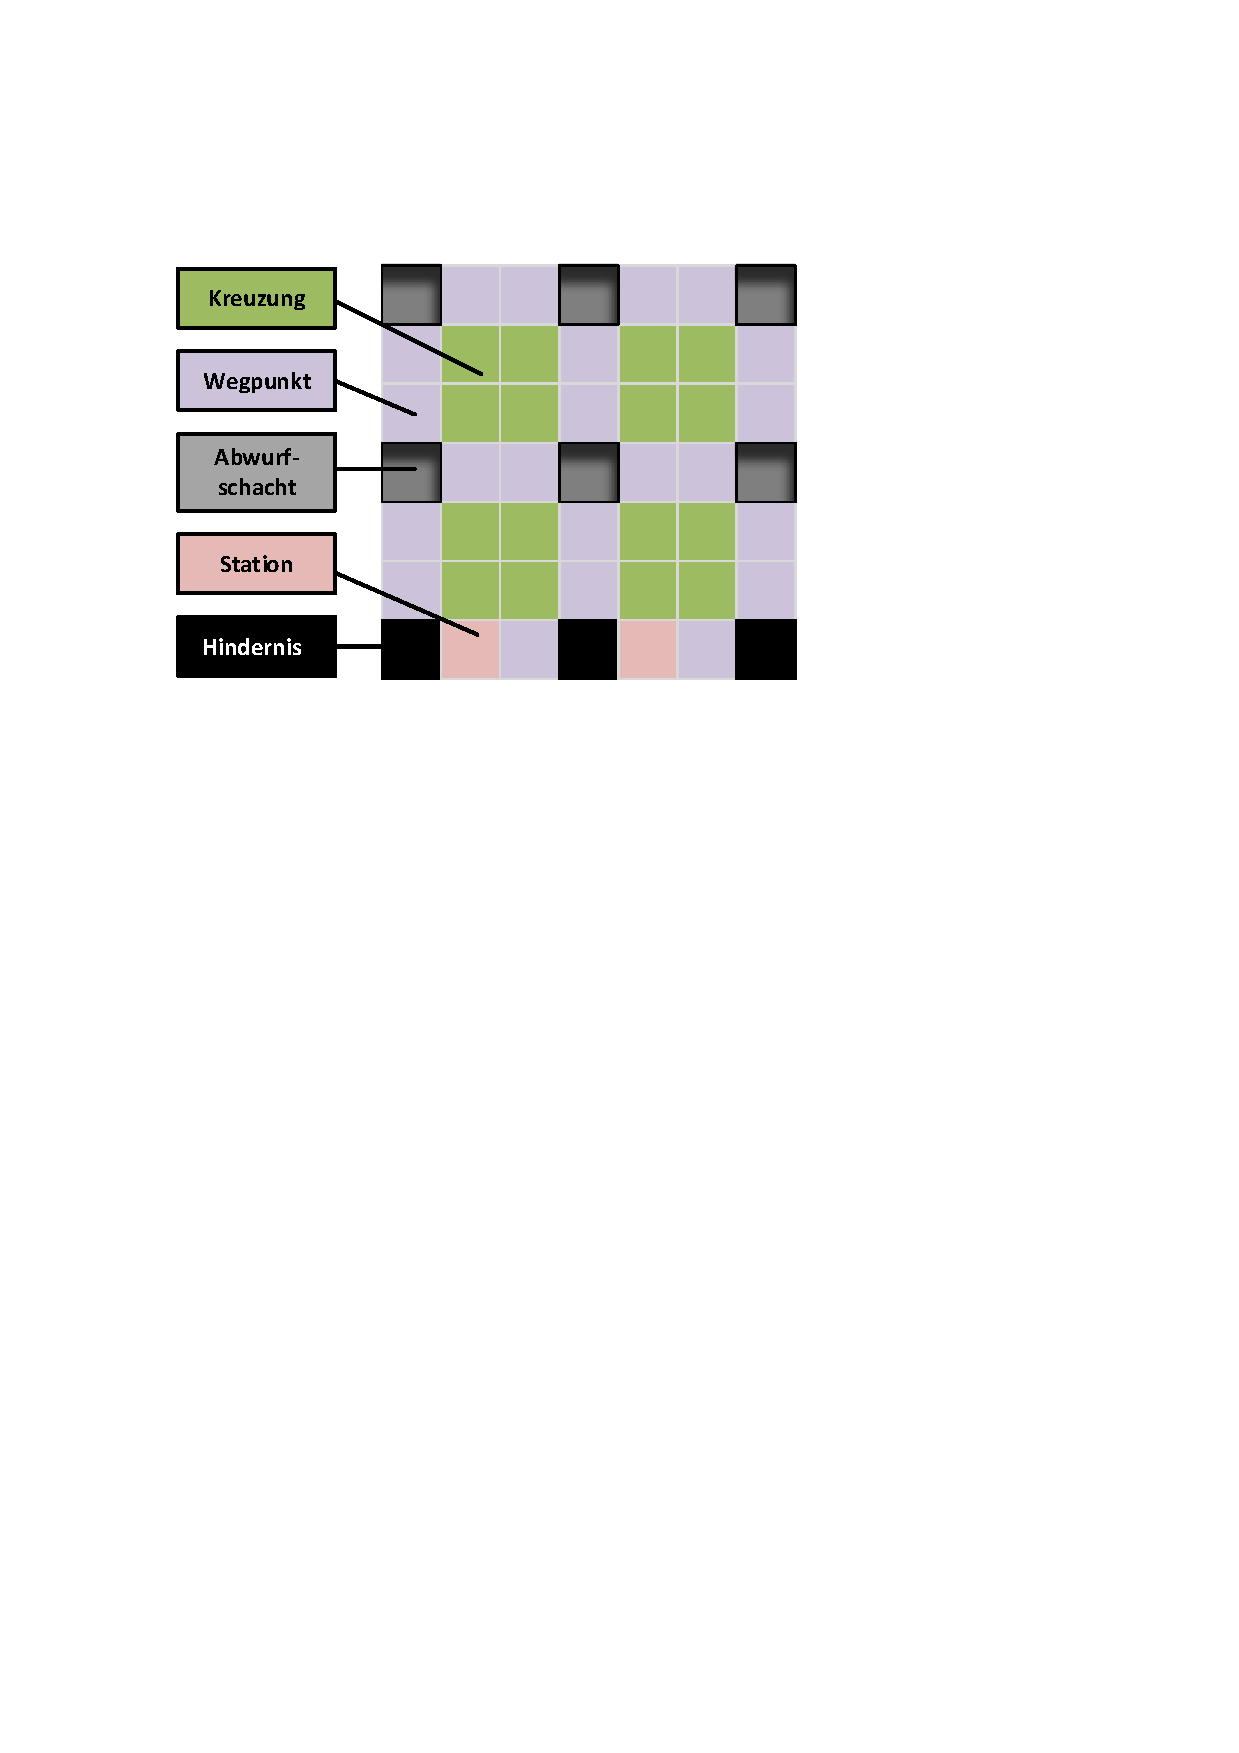
\includegraphics[scale=0.8]{fieldtypes_grid}
	\caption{Übersicht über den Aufbau der Paketsortieranlage und die wichtigsten Begriffe. Die Farben der Felder kennzeichnen die Positionstypen, die von den Robotersensoren erkannt werden können.}
	\label{fig:grid_field_naming}
\end{figure}



\begin{figure}
    \centering
	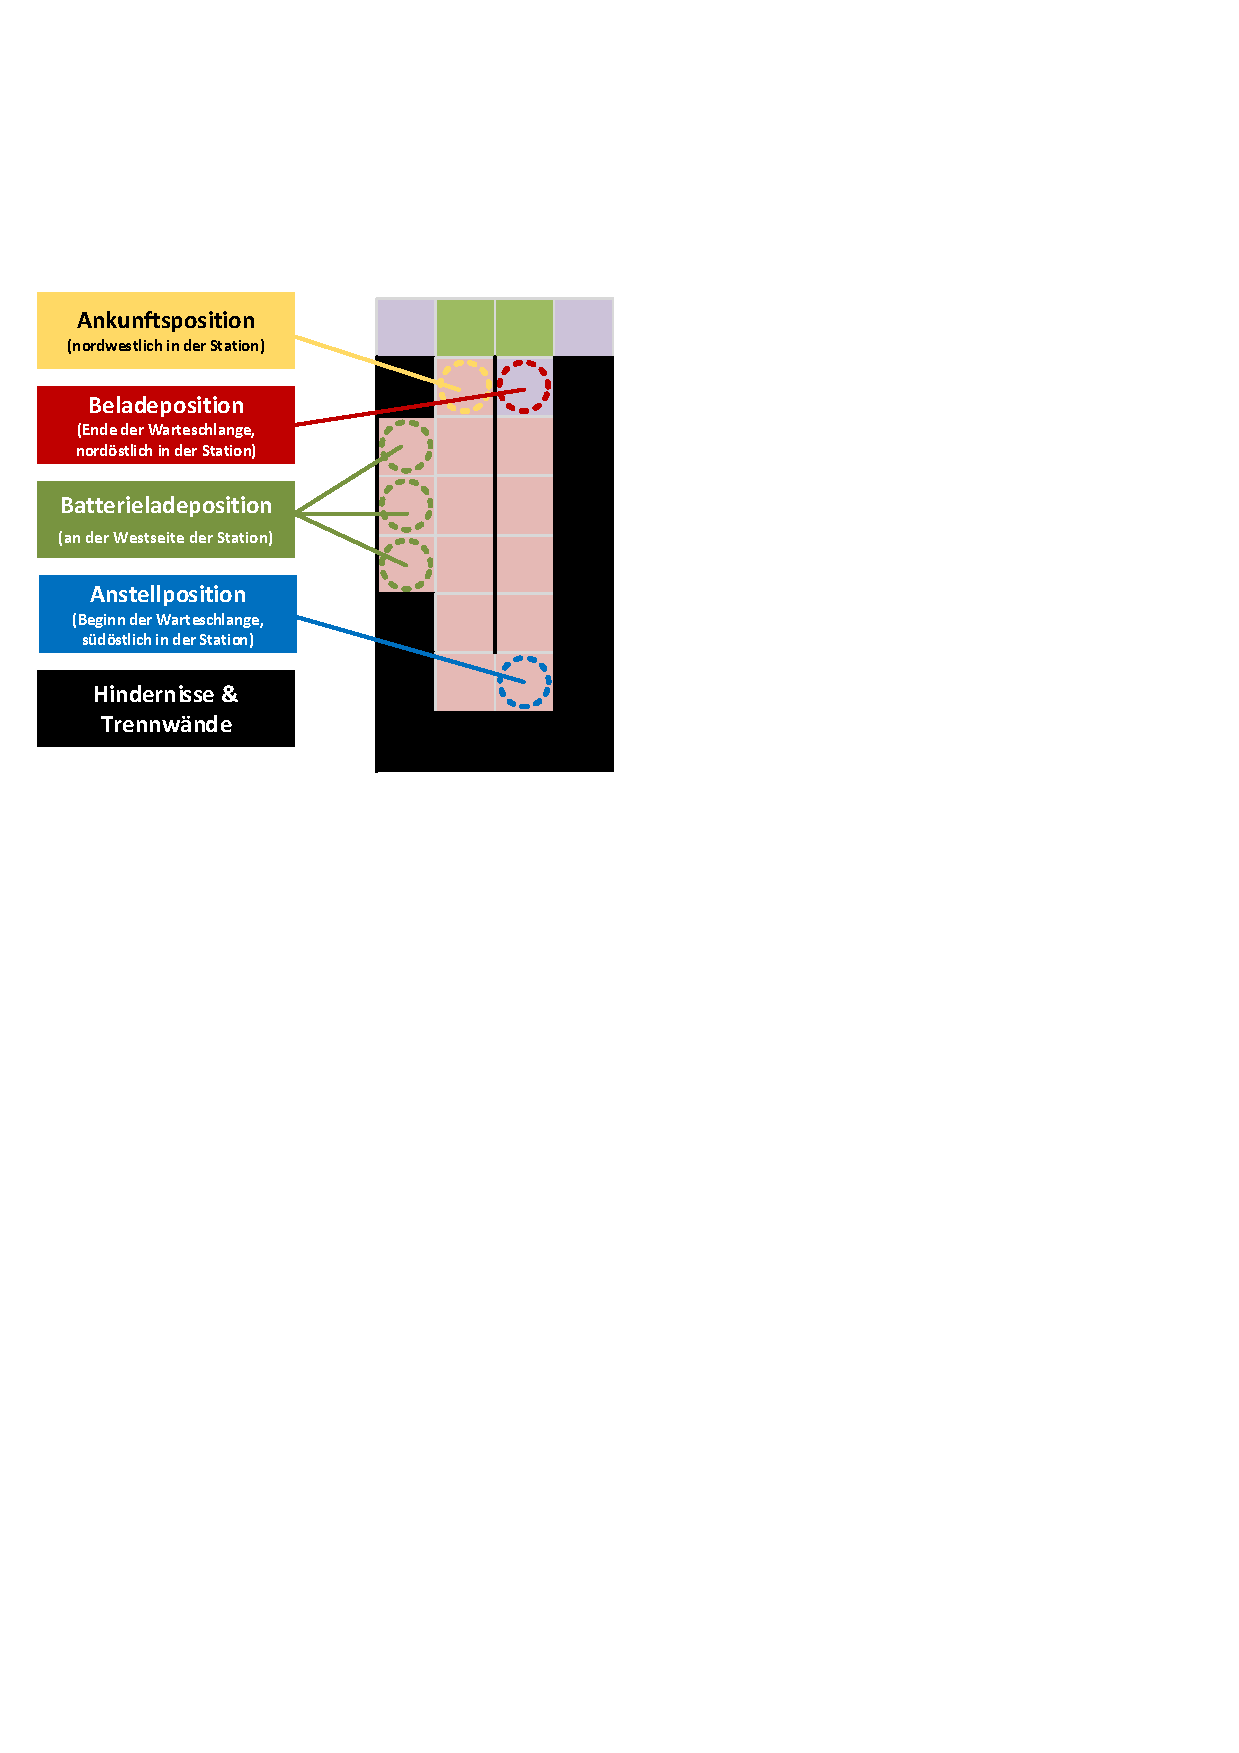
\includegraphics[scale=0.8]{fieldtypes_station}
	\caption{Übersicht über den Aufbau einer Station in der Paketsortieranlage, inklusive der wichtigsten Bezeichnungen für die einzelnen Positionen, zu denen ein Roboter disponiert werden kann.}
	\label{fig:grid_station_naming}
\end{figure}

Die Struktur der Paketsortieranlage ist in \autoref{fig:grid_field_naming} dargestellt und im Folgenden beschrieben. 
Die (potentiell beliebig große) Fläche der Sortieranlage ist in quadratische Felder eingeteilt, die jeweils ganzzahlige Koordinaten haben und gezielt von den Robotern angefahren werden können. 
Die Felder sind jeweils groß genug, so dass ein Roboter sich auf der Stelle drehen kann, ohne mit den Robotern auf den Nachbarfeldern zu kollidieren.

Auf der Fläche der Sortieranlage befinden sich in regelmäßigen Abständen \emph{Abwurfschächte}. 
Zwischen je zwei Abwurfschächten sind immer zwei Felder frei. 
Die Streifen zwischen den Schächten bilden \emph{Straßen}, die aus \emph{Kreuzungen} und sogenannten \emph{Wegpunkten} bestehen.
Auf den Straßen herrscht \textbf{strikter Rechtsverkehr}. 
An Kreuzungen gilt die \textbf{Vorfahrtsregel \enquote{Rechts vor Links}}. 
Durch diese beiden Regeln können autonom fahrende Roboter Kollisionen und Deadlocks vermeiden.

An der Südseite der Sortieranlage befinden sich nebeneinander aufgereiht mehrere \emph{Stationen}, die der in \autoref{fig:grid_station_naming} gezeigten Struktur entsprechen.
Als Übergang zwischen einer Station und der restlichen Fläche der Sortieranlage dienen zwei Felder: die \emph{Ankunftsposition}, auf der rechtsseitig fahrende Roboter aus dem freien Verkehr ankommen, und die \emph{Beladeposition}, von der aus sich Roboter in den Verkehr einordnen können.

Innerhalb einer Station befindet sich links eine Strecke, an der die \emph{Batterieladepositionen} liegen. 
Fährt ein Roboter rückwärts in die Batterieladeposition hinein, beginnt die Aufladung automatisch. 
Die serverseitige Roboterdisposition stellt sicher, dass diese Strecke links der Station immer nur von einem Roboter befahren wird, so dass beim Aus- und Einparken nicht auf Kollisionen geachtet werden muss.

Auf der rechten Seite der Station befindet sich eine \emph{Warteschlange}, in der Roboter darauf warten, beladen zu werden. 
Die vorderste Position der Warteschlange ist die Beladeposition und zugleich der Eintrittspunkt in den regulären Verkehr. 
Da sich die Beladeposition vor einer Kreuzung befindet, erkennt ein darauf stehender Roboter sie als einen Wegpunkt. 
Die Roboter werden zuerst immer zur \emph{Anstellposition} (Ende der Warteschlange) dirigiert und erst danach zur Beladeposition.

Aufgrund von Trennwänden zwischen der rechten und der linken Hälfte der Station, erkennen die Roboter die entsprechenden Nachbarfelder als blockiert. 
Gleiches gilt für \emph{Hindernisse} und Abwurfschächte.


	%!TEX root = ../../entwurfsprojekt2_entwurfsdokument.tex

\section{Innere Struktur der Komponenten}
\label{sec:struktur}


\subsection{Struktur des Roboterteilsystems (Komponente \texttt{LogisticsRobot})}

\begin{figure}[h]
	\centering
	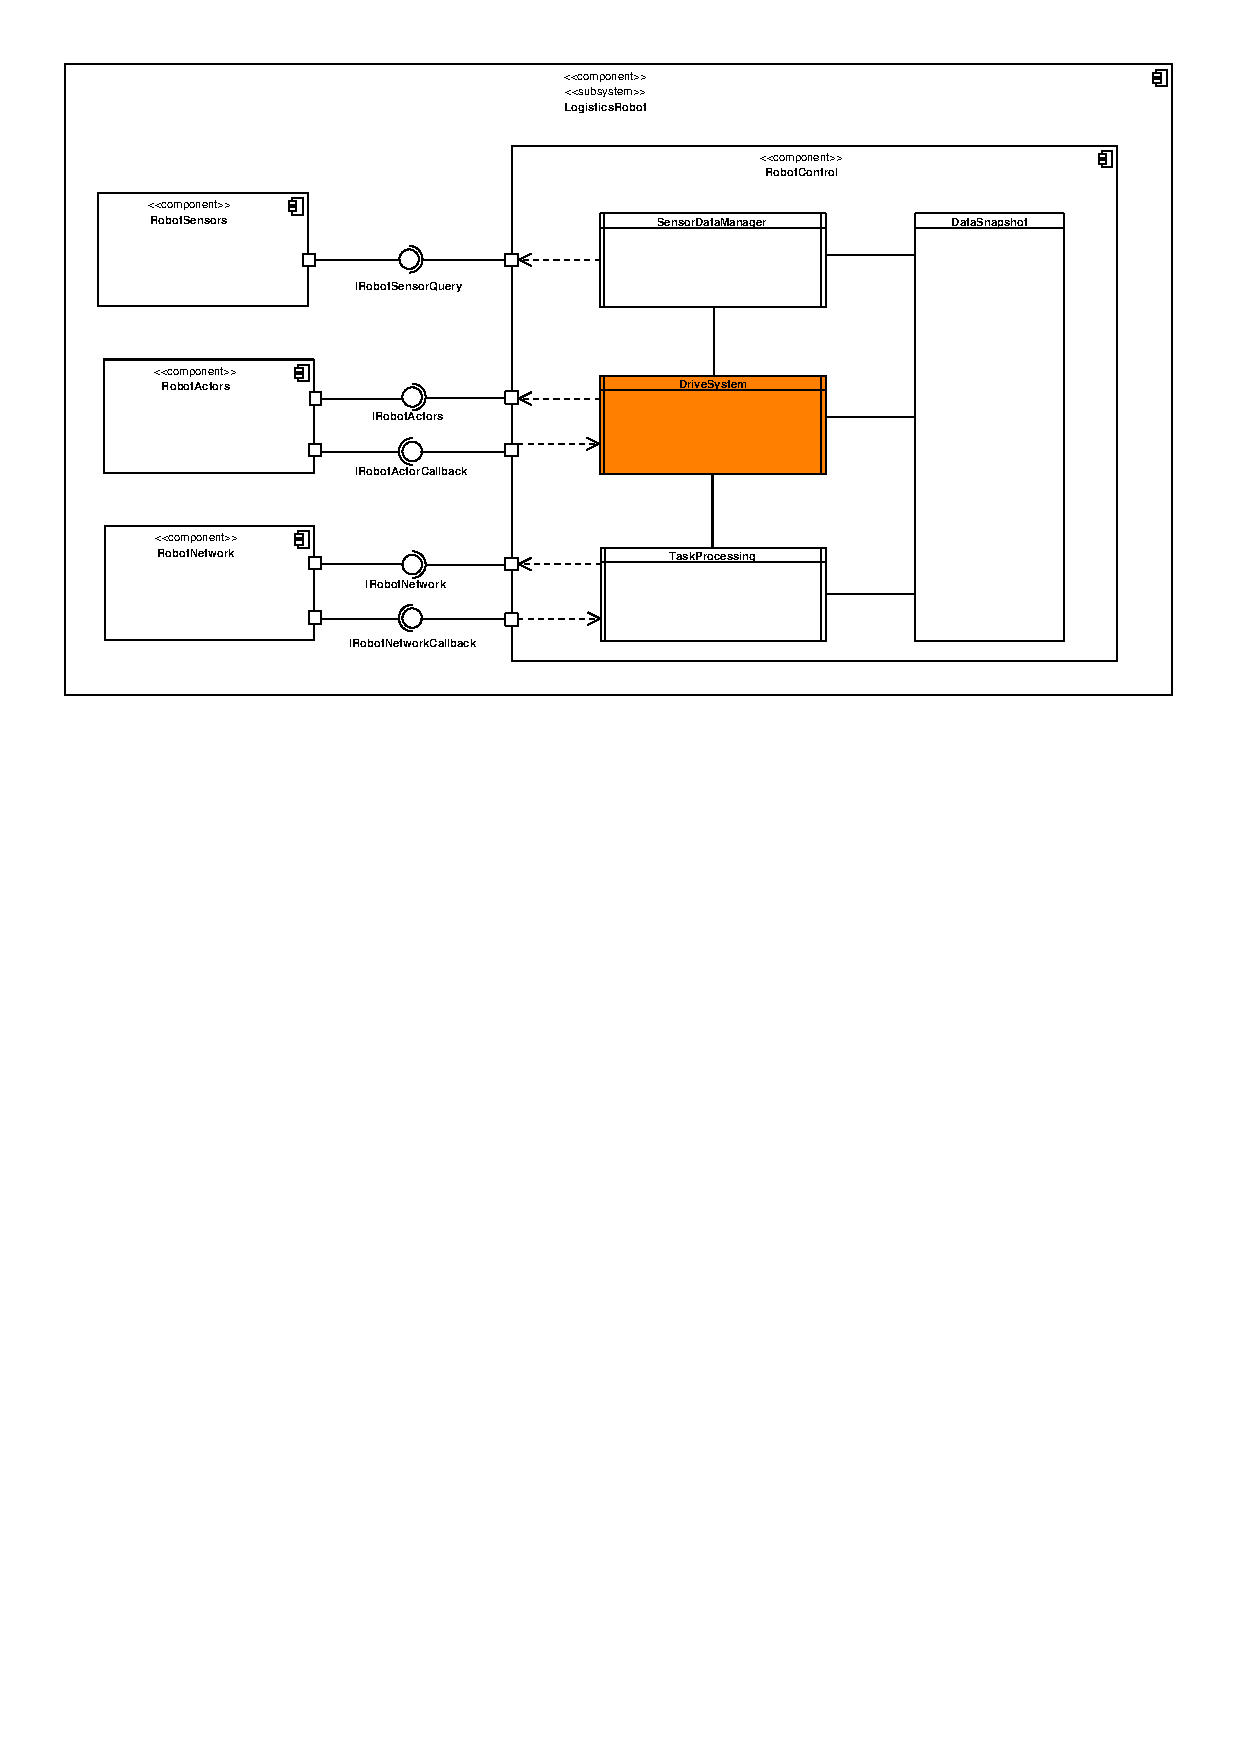
\includegraphics[width=\textwidth]{robot_component_internals}
	\caption{Architektur des Roboterteilsystems.}
	\label{fig:robot_component}
\end{figure}



Auf allen Robotern läuft die gleiche Software (beschrieben durch die gegebene Komponente \texttt{LogisticsRobot}), die sich aus vier Unterkomponenten zusammensetzt (siehe \autoref{fig:robot_component}).

Die Unterkomponente \texttt{RobotControl} ist die zentrale Unterkomponente, die den Roboter steuert. 
Sie enthält die aktive Klasse \texttt{DriveSystem}, welche Zugriff auf die Aktuatoren hat und dadurch das Fahrverhalten eines Roboters bestimmt.
Außerdem beinhaltet die Unterkomponente \texttt{RobotControl} die Klasse \texttt{SensorDataManager} für das Abrufen von Sensordaten, die Klasse \texttt{DataSnapshot} für Speicherung der Sensordaten und die aktive Klasse \texttt{TaskProcessing} für das Empfangen von Aufträgen.


Zur eigentlichen Bewegung stehen physische Aktuatoren zur Verfügung, die von der Unterkomponente \texttt{RobotActors} kontrolliert werden.
Neben Aktuatoren sind auch Sensoren verfügbar. 
Die Messwerte dieser Sensoren stellt die Unterkomponente \texttt{RobotSensors} zur Verfügung.
Die Unterkomponente \texttt{RobotNetwork} wickelt die Kommunikation eines Roboters mit den anderen Teilsystemen ab.
	%!TEX root = ../../entwurfsprojekt2_entwurfsdokument.tex

\begin{figure}[h]
	\centering
	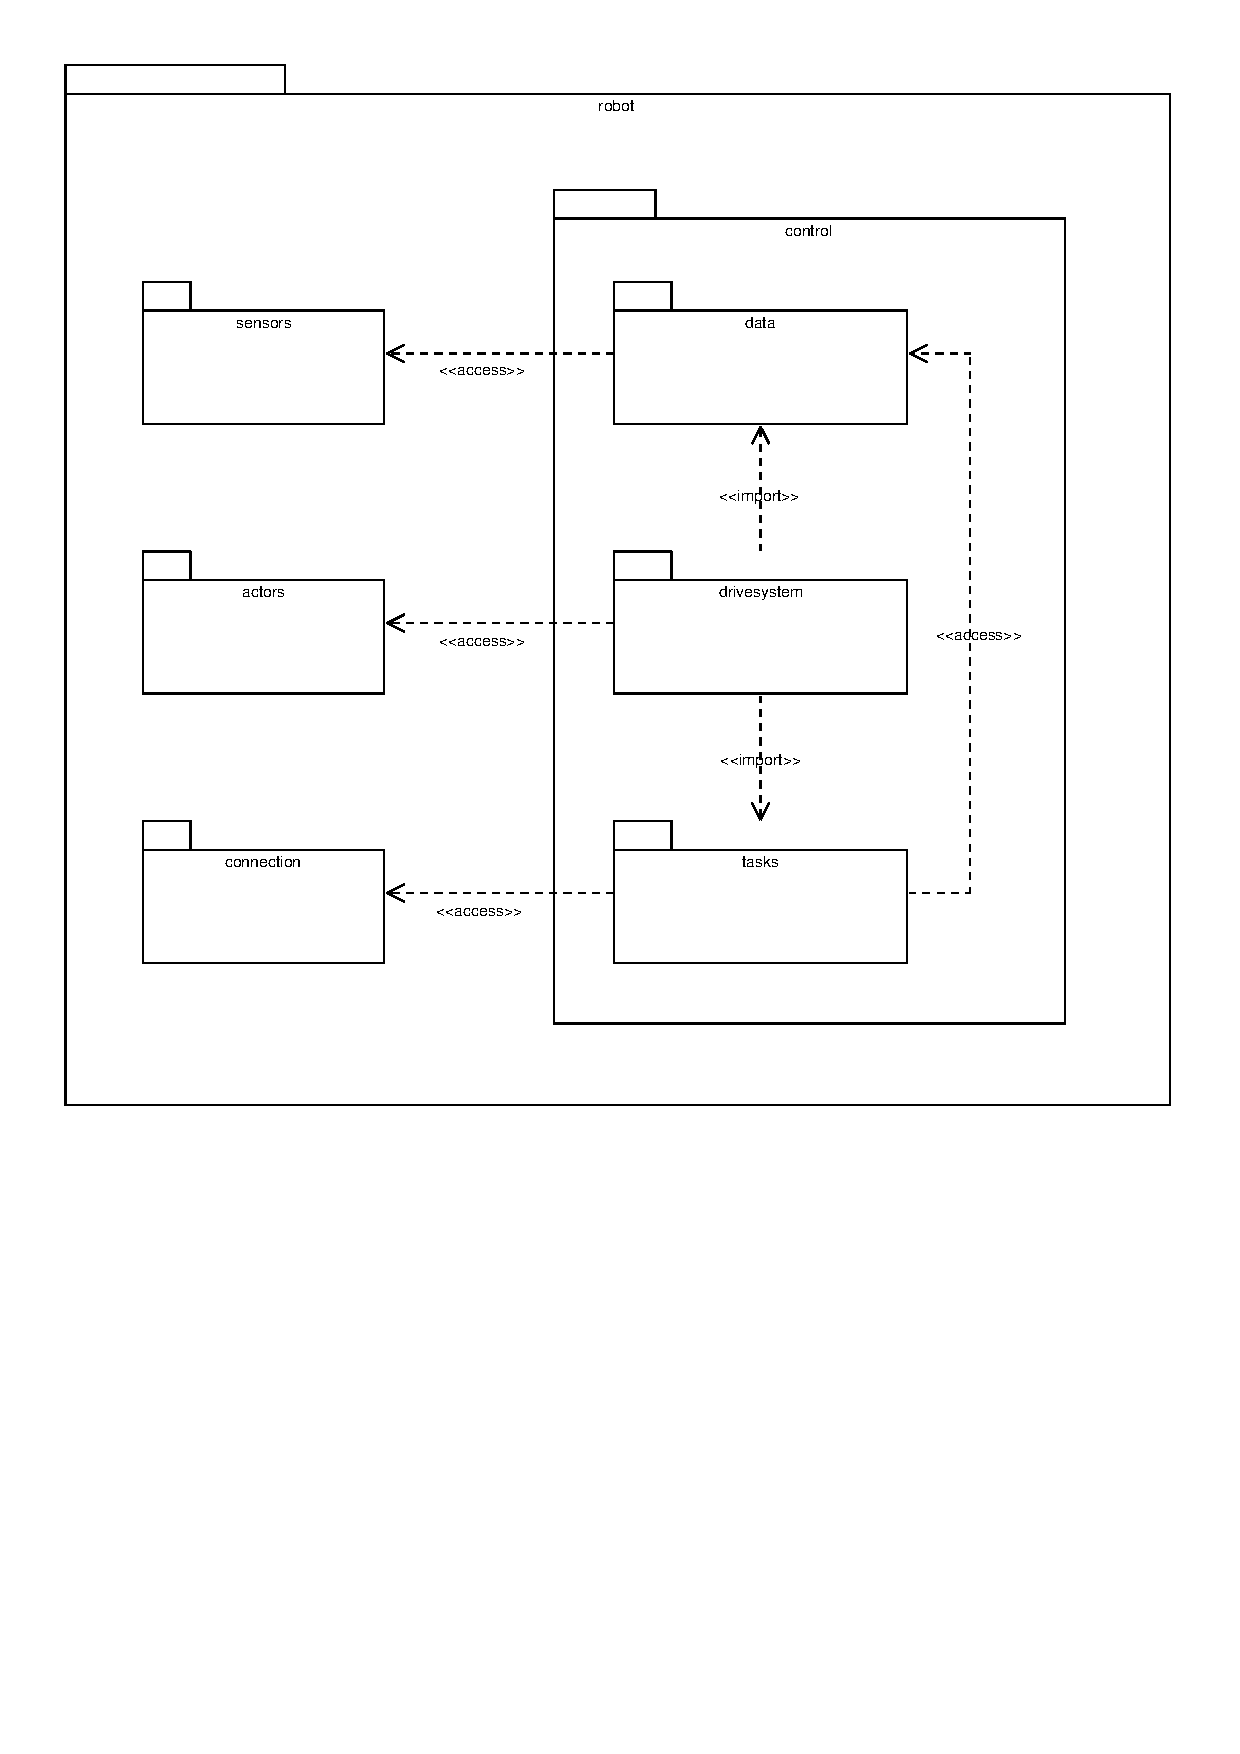
\includegraphics[width=0.7\textwidth]{robot_packages}
	\caption{Paketstruktur des Roboterteilsystems.}
	\label{fig:robot_packages}
\end{figure}

\section{Paketstruktur}
\label{sec:pakete}



Die Inhalte der Komponente \texttt{LogisticsRobot} werden in dem Paket \texttt{robot} implementiert.
Dieses enthält für jede der vier Unterkomponenten \texttt{RobotControl}, \texttt{RobotActors}, \texttt{RobotSensors} und \texttt{RobotNetwork} ein Unterpaket. 
Die Unterpakete \texttt{actors}, \texttt{sensors} und \texttt{connection} sind nicht weiter unterteilt, während das Unterpaket \texttt{control} noch einmal in die Unterpakete \texttt{data}, \texttt{drivesystem} und \texttt{tasks} aufgeteilt ist.

Die sich ergebende Paketstruktur mit den Abhängigkeiten zwischen den einzelnen Paketen ist in \autoref{fig:robot_packages} dargestellt.

	%!TEX root = ../../entwurfsprojekt2_entwurfsdokument.tex

\section{Paketdetails}
\label{sec:details}

In diesem Abschnitt werden für das Paket \texttt{robot.control.drivesystem} Details zur Implementierung gegeben.

Im Folgenden wird eine vollständige Spezifikation aller Klassen gegeben, die entweder direkt im Paket \texttt{drivesystem} implementiert werden oder aus anderen Paketen per Import- oder Zugriffsbeziehung eingebunden werden.
Diese Klassen sind in \autoref{fig:robot_classes} gemeinsam dargestellt.

\begin{figure}[h]
	\centering
	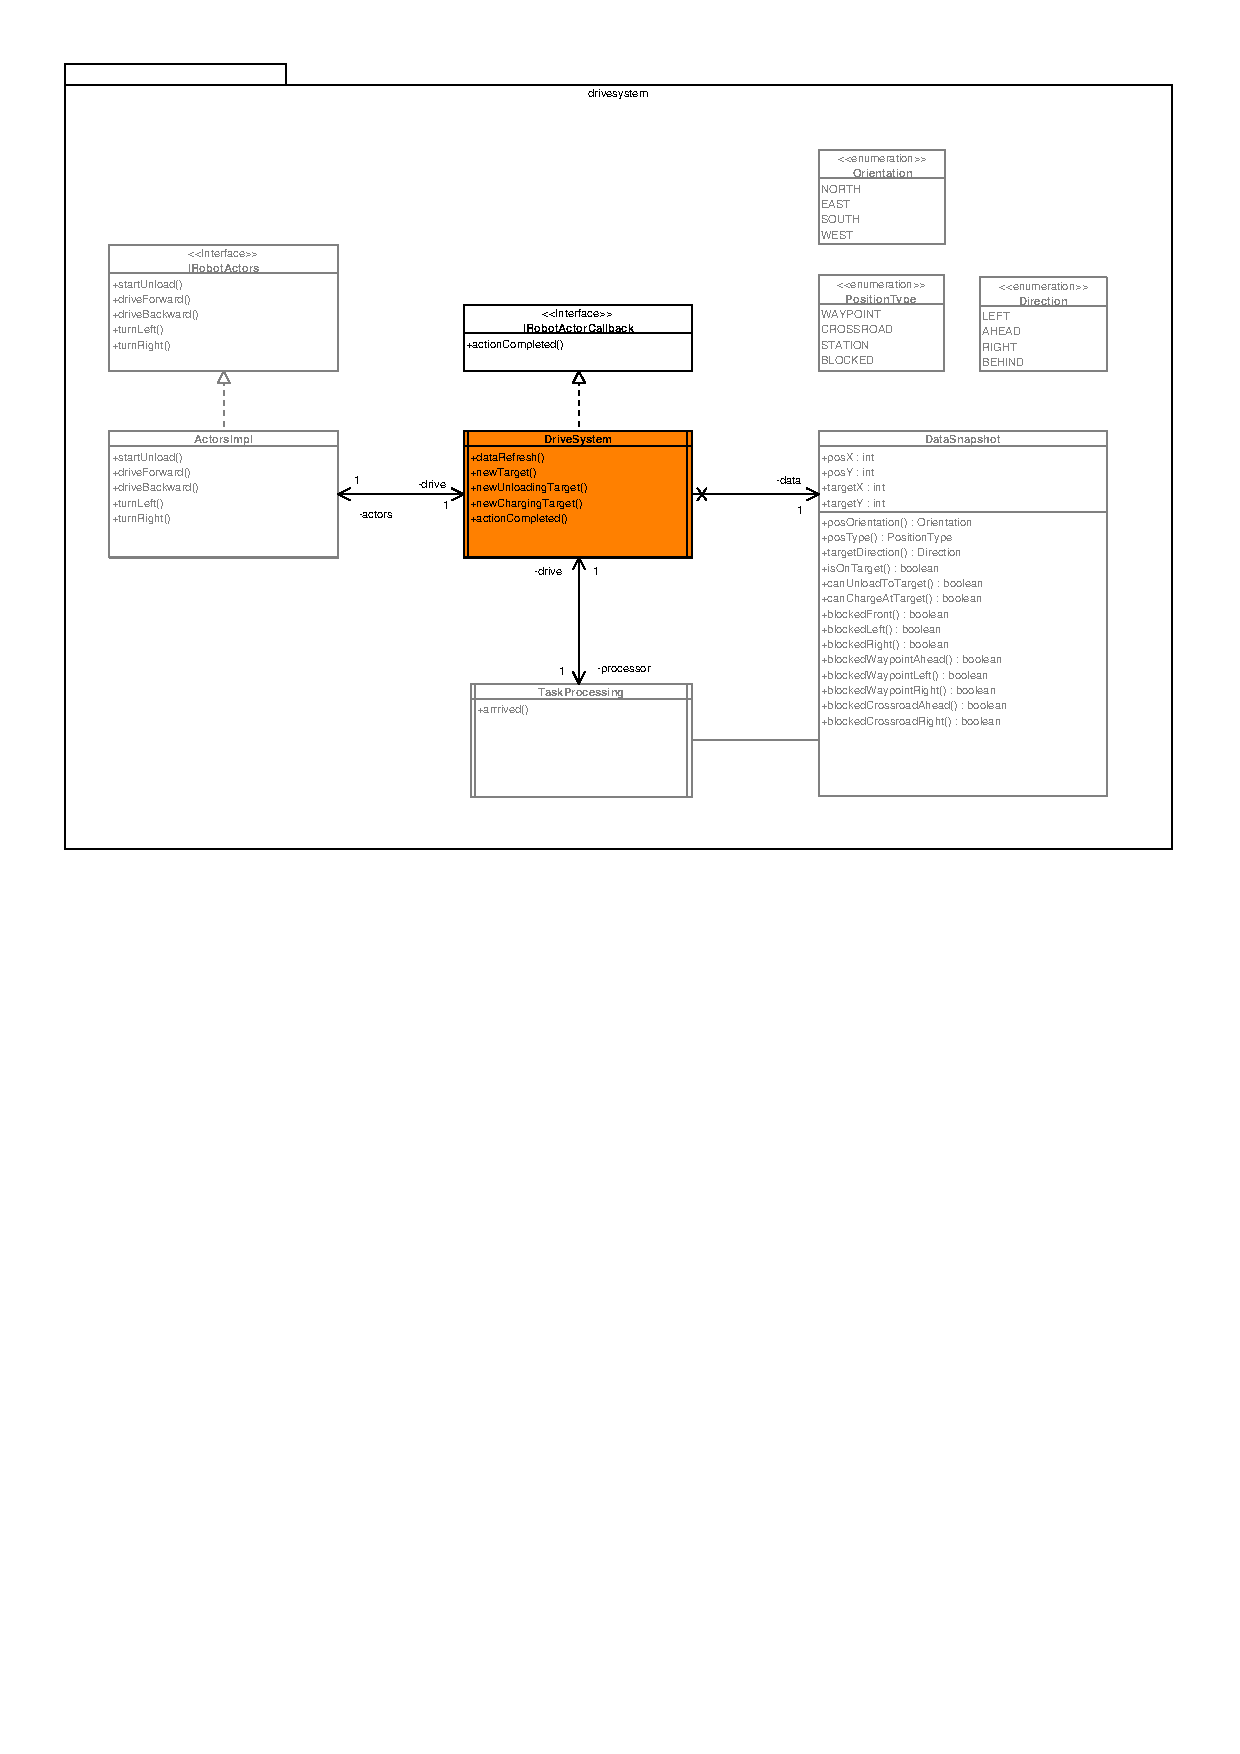
\includegraphics[width=\textwidth]{img/robot_classes}
	\caption{Inhalte des Pakets \texttt{robot.control.drivesystem}. Aus anderen Paketen per Import- oder Zugriffsbeziehung eingebundene Inhalte sind grau markiert.}
	\label{fig:robot_classes}
\end{figure}


\subsection{Klasse \texttt{DriveSystem}}
\label{class:drive}

Die aktive Klasse \texttt{DriveSystem} erhält Aufträge von der \nameref{class:tasks} und setzt diese (basierend auf den aktuellen Sensordaten) in Bewegungsbefehle um. 
Dieses Fahrverhalten soll durch ein Statechart beschrieben werden.

Die Klasse \texttt{DriveSystem} implementiert fünf Methoden mit öffentlicher Sichtbarkeit, die als Eingaben für das Statechart fungieren. 
Das jeweils beschriebene Verhalten ist mithilfe eines gemeinsamen Statecharts umzusetzen.


\subsubsection{Methode \texttt{newTarget()}}
\label{method:newtarget}

Die Methode \texttt{newTarget()} wird aufgerufen, um der Klasse \texttt{DriveSystem} mitzuteilen, dass in der \nameref{class:data} neue Zielkoordinaten hinterlegt wurden.
Die \nameref{class:tasks} ist verantwortlich für das Hinterlegen der Zielkoordinaten und das Aufrufen der Methode \texttt{newTarget()}.

Das Statechart soll als Reaktion auf diesen Methodenaufruf so lange Bewegungsbefehle an die \nameref{class:actors} senden, bis das hinterlegte Ziel erreicht wurde. 
Das Erreichen des Ziels kann durch die \nameref{method:ontarget} der \nameref{class:data} überprüft werden.

Die Bewegungsbefehle sollen so erteilt werden, dass mithilfe der Sensordaten Verkehrsregeln eingehalten und Kollisionen und Deadlocks der Roboter vermieden werden. 

Es ist davon auszugehen, dass die gegebenen Zielkoordinaten immer in einer Station oder auf einem Wegpunkt sind. 
Ist das Ziel wider Erwarten auf einer Kreuzung, ist diese nach Ankunft sofort zu verlassen.

Nach erfolgreicher Erfüllung des Fahrauftrages soll bei der \nameref{class:tasks} die \nameref{method:arrived} aufgerufen werden. Das Statechart soll keine weiteren Bewegungen veranlassen bis der Erhalt eines neuen Ziels gemeldet wird.



\subsubsection{Methode \texttt{newUnloadingTarget()}}
\label{method:unloadingtarget}

Ähnlich zu der \nameref{method:newtarget}, dient auch die Methode \texttt{newUnloadingTarget()} dazu, die Klasse \texttt{DriveSystem} auf neue Zielkoordinaten hinzuweisen.

Das Statechart soll als Reaktion auf diesen Methodenaufruf das hinterlegte Ziel anfahren, wie es auch bei der \nameref{method:newtarget} passiert.
Allerdings handelt es sich hier bei den Zielkoordinaten um die Koordinaten eines Abwurfschachtes, so dass die Fahrt bereits \emph{neben} diesem Schacht beendet werden soll. 
Ob der Roboter sich neben dem anzufahrenden Abwurfschacht befindet, kann mit der \nameref{method:nexttounload} der \nameref{class:data} überprüft werden.

Nach der Ankunft am Schacht und \emph{vor} der Erfolgsmeldung durch die \nameref{method:arrived} muss das Paket mithilfe der \nameref{method:unload} in den Schacht abgeworfen werden.


\subsubsection{Methode \texttt{newChargingTarget()}}
\label{method:chargingtarget}

Auch die Methode \texttt{newChargingTarget()} ist eine Sondervariante der \nameref{method:newtarget}, die die Klasse \texttt{DriveSystem} auf neue Zielkoordinaten hinweist.

Die Zielkoordinaten beschreiben in diesem Fall eine Batterieladeposition. 
In diese Batterieladeposition muss rückwärts eingeparkt werden, um die Batterieladevorrichtung nicht zu beschädigen. 
Um das Einparkmanöver zu beginnen, kann mit der \nameref{method:nexttocharger} der \nameref{class:data} überprüft werden, ob der Roboter sich genau neben der anzufahrenden Batterieladeposition befindet.


\subsubsection{Methode \texttt{actionCompleted()}}
\label{method:completed}

Die Methode \texttt{actionCompleted()} teilt der Klasse \texttt{DriveSystem} mit, dass eine laufende Bewegung beendet wurde.
Der Aufruf dieser Methode signalisiert dem Statechart, dass die \nameref{class:actors} für einen weiteren Bewegungsbefehl bereit ist.


\subsubsection{Methode \texttt{dataRefresh()}}
\label{method:refresh}

Die Methode \texttt{dataRefresh()} wird aufgerufen, um der Klasse \texttt{DriveSystem} mitzuteilen, dass die Sensordaten in der \nameref{class:data} aktualisiert wurden. 
Wenn der Roboter ein Ziel hat \emph{und} aktuell keine Bewegung ausgeführt wird, soll das Statechart als Reaktion auf diesen Methodenaufruf die vorliegenden Sensordaten prüfen und, falls möglich, eine Bewegung der Aktuatoren veranlassen.

Die Methode \texttt{dataRefresh()} wird mit hoher Frequenz aufgerufen und kann daher zusätzlich genutzt werden, um innerhalb des Statecharts periodische Aktivitäten auszulösen.



\subsection{Klasse \texttt{ActorsImpl}}
\label{class:actors}

Die Klasse \texttt{ActorsImpl} ist ein Teil der Komponente \texttt{RobotActors} und realisiert das von der Komponente nach außen angebotene Interface \texttt{IRobotActors}.
Die Klasse \texttt{ActorsImpl} wird im Paket \texttt{robot.actors} implementiert.

Es stehen insgesamt fünf durch das Interface \texttt{IRobotActors} vorgegebene öffentliche Methoden zur Verfügung. 
Jede dieser Methoden wird zum Auslösen eines bestimmten Bewegungsbefehls genutzt.
Wenn in einem Zustandsübergang mehrere Bewegungsbefehle aufgerufen werden, wird nur einer davon ausgelöst.


\subsubsection{Methode \texttt{driveForward()}}
\label{method:drive}

Die Methode \texttt{driveForward()} lässt den Roboter ein einzelnes Feld nach vorne fahren. 
Nach der Ankunft wird die \nameref{method:completed} der \nameref{class:drive} aufgerufen.
Kommt ein \texttt{driveForward()} Aufruf, während bereits eine Bewegung läuft, wird dieser verworfen.

Die Methode \texttt{driveForward()} nimmt keine Rücksicht auf eventuelle Hindernisse.


\subsubsection{Methode \texttt{driveBackward()}}
\label{method:driveback}

Die Methode \texttt{driveBackward()} lässt den Roboter ein einzelnes Feld nach hinten fahren.~Nach der Ankunft wird die \nameref{method:completed} der \nameref{class:drive} aufgerufen.
Kommt ein \texttt{driveBackward()} Aufruf, während bereits eine Bewegung läuft, wird dieser verworfen.

Die Methode \texttt{driveBackward()} nimmt keine Rücksicht auf eventuelle Hindernisse.


\subsubsection{Methode \texttt{turnLeft()}}
\label{method:turnleft}

Die Methode \texttt{turnLeft()} lässt den Roboter auf einem Feld um 90$^{\circ}$ nach links rotieren. 
Nach dem Ende der Rotation wird die \nameref{method:completed} der \nameref{class:drive} aufgerufen.
Kommt ein \texttt{turnLeft()} Aufruf, während bereits eine Bewegung läuft, wird dieser verworfen.


\subsubsection{Methode \texttt{turnRight()}}
\label{method:turnright}

Die Methode \texttt{turnRight()} lässt den Roboter auf einem Feld um 90$^{\circ}$ nach rechts rotieren.~Nach dem Ende der Rotation wird die \nameref{method:completed} der \nameref{class:drive} aufgerufen.
Kommt ein \texttt{turnRight()} Aufruf, während bereits eine Bewegung läuft, wird dieser verworfen.

\enlargethispage{2\baselineskip}

\subsubsection{Methode \texttt{startUnload()}}
\label{method:unload}

Die Methode \texttt{startUnload()} lässt den Roboter seine Ladefläche nach rechts kippen, so dass ein eventuell geladenes Paket abgeworfen wird. 
Nach dem Abwurf wird auch hier die \nameref{method:completed} aufgerufen.
Kommt ein \texttt{startUnload()} Aufruf, während bereits eine Bewegung läuft, wird dieser verworfen.

Die Methode \texttt{startUnload()} kontrolliert nicht die Ausrichtung des Roboters zum Abwurfschacht.




\subsection{Klasse \texttt{TaskProcessing}}
\label{class:tasks}

Die aktive Klasse \texttt{TaskProcessing} ist ein Teil der Komponente \texttt{RobotControl} und wird im Paket \texttt{robot.control.tasks} implementiert. 
Diese Klasse verantwortet die Netzwerkkommunikation mit anderen Teilsystemen.

Die Klasse \texttt{TaskProcessing} erhält von einer externen Stelle die Aufträge. 
Beim Eingang eines Auftrages trägt die Klasse \texttt{TaskProcessing} die neuen Zielkoordinaten in der \nameref{class:data} ein und informiert die \nameref{class:drive} über den Eingang neuer Zielkoordinaten mit einem Aufruf der \nameref{method:newtarget}, der \nameref{method:unloadingtarget} oder der \nameref{method:chargingtarget}.

Für Rückmeldungen der \nameref{class:drive} stellt die Klasse \texttt{TaskProcessing} zudem eine öffentlich sichtbare Methode \texttt{arrived()} zur Verfügung.


\subsubsection{Methode \texttt{arrived()}}
\label{method:arrived}

Die Methode \texttt{arrived()} informiert die Klasse \texttt{TaskProcessing} darüber, dass das hinterlegte Ziel von der \nameref{class:drive} erreicht wurde (inkl. der Fälle, bei denen der Roboter ein Paket abwirft bzw. zum Aufladen der Batterie einparkt).
Der Aufruf der Methode \texttt{arrived()} löst aus, dass die Klasse \texttt{TaskProcessing} den Erfolg über das Netzwerk meldet und dann ggf. einen weiteren Auftrag für den Roboter erhalten kann.



\subsection{Klasse \texttt{DataSnapshot}}
\label{class:data}

Die Klasse \texttt{DataSnapshot} ist ein Teil der Komponente \texttt{RobotControl} und wird im Paket \texttt{robot.control.data} implementiert. 
Diese Klasse dient der Speicherung der jeweils aktuellen Sensordaten.

Um dem Statechart möglichst präzisen Zugriff auf die Sensordaten zu ermöglichen, implementiert die Klasse \texttt{DataSnapshot} eine Reihe von Methoden, die die Sensordaten präzise interpretieren.
Diese Methoden lassen sich grob sortieren nach Zielüberprüfung, Orientierung im Raum und Hinderniserkennung.

\enlargethispage{2\baselineskip}

\subsection*{Methoden zur Zielüberprüfung}


\subsubsection{Methode \texttt{isOnTarget()}}
\label{method:ontarget}

Die Methode \texttt{isOnTarget()} gibt einen \texttt{boolean} zurück. 
Die Rückgabe der Methode ist genau dann wahr, wenn die aktuelle Position des Roboters der Zielposition genau entspricht.


\subsubsection{Methode \texttt{canUnloadToTarget()}}
\label{method:nexttounload}

Die Methode \texttt{canUnloadToTarget()} gibt einen \texttt{boolean} zurück. 
Die Rückgabe der Methode ist genau dann wahr, wenn die Zielposition ein Abwurfschacht ist und der Roboter sich genau ein Feld horizontal oder vertikal neben dieser Zielposition befindet, so dass er das Paket in den Abwurfschacht abwerfen kann.


\subsubsection{Methode \texttt{canChargeAtTarget()}}
\label{method:nexttocharger}

Die Methode \texttt{canChargeAtTarget()} gibt einen \texttt{boolean} zurück. 
Die Rückgabe der Methode ist genau dann wahr, wenn die Zielposition eine Batterieladeposition ist und der Roboter sich genau ein Feld rechts von dieser Zielposition befindet, so dass er rückwärts einparken kann.


\subsection*{Methoden zur Orientierung im Raum}


\subsubsection{Methode \texttt{posType()}}

Die Methode \texttt{posType()} gibt einen \texttt{PositionType} aus der entsprechenden Enumeration zurück.
Die \texttt{PositionType}-Enumeration ist in \autoref{fig:robot_classes} gegeben und enthält als mögliche Werte \texttt{STATION}, \texttt{WAYPOINT}, \texttt{CROSSROAD} und \texttt{BLOCKED} (für Hindernisse).
Mithilfe eines \texttt{PositionType}-Wertes kann festgestellt werden, auf welcher Art von Feld sich der Roboter derzeit befindet. 


\subsubsection{Methode \texttt{posOrientation()}}

Die Methode \texttt{posOrientation()} gibt eine \texttt{Orientation} aus der entsprechenden Enumeration zurück.
Die \texttt{Orientation}-Enumeration ist in \autoref{fig:robot_classes} gegeben und enthält als mögliche Werte \texttt{NORTH}, \texttt{SOUTH}, \texttt{EAST} und \texttt{WEST}.
Mithilfe eines \texttt{Orientation}-Wertes kann festgestellt werden, in welche Himmelsrichtung ein Roboter ausgerichtet ist. 
%Die Rückgabe ist vom Typ \texttt{Orientation} und kann die Werte  \texttt{NORTH}, \texttt{EAST}, \texttt{SOUTH} oder \texttt{WEST} haben.

\subsubsection{Methode \texttt{targetDirection()}}
\label{method:targetdirection}

Die Methode \texttt{targetDirection()} gibt eine \texttt{Direction} aus der entsprechenden Enumeration zurück.
Die \texttt{Direction}-Enumeration ist in \autoref{fig:robot_classes} gegeben und enthält als mögliche Werte \texttt{AHEAD}, \texttt{BEHIND}, \texttt{LEFT} und \texttt{RIGHT}.
Mithilfe eines \texttt{Direction}-Wertes kann festgestellt werden, in welcher Richtung (ausgehend von der Fahrtrichtung des Roboters) sich das aktuelle Ziel befindet. 
%Die Methode \texttt{targetDirection()} gibt zurück, in welche Richtung (ausgehend von der Fahrtrichtung des Roboters) sich das aktuelle Ziel befindet.
%Die Rückgabe ist vom Typ \texttt{Direction} und kann die Werte  \texttt{AHEAD}, \texttt{LEFT}, \texttt{RIGHT} oder \texttt{BEHIND} haben.

Die Methode \texttt{targetDirection()} nimmt bei ihrer Rückgabe Rücksicht auf das Rechtsfahrgebot, wenn Roboter auf einer Kreuzung oder einem Wegpunkt stehen. 
Bei den Zielen, die schräg vorne bzw. schräg hinten liegen, wird immer \texttt{AHEAD} bzw. \texttt{BEHIND} zurückgegeben. 
Die Rückgaben \texttt{LEFT} oder \texttt{RIGHT} kommen erst dann, wenn ein einmaliges Abbiegen genügt, um einen direkten Weg zum Ziel zu haben.

Die Rückgaben der Methode \texttt{targetDirection()} hängen von der Art von Feld ab, auf dem sich der Roboter befindet.
%Um die entsprechenden Rückgaben zu realisieren gibt die Methode \texttt{targetDirection()} sehr unterschiedliche Rückgaben je nach Art von Feld auf dem ein Roboter steht.
Die schematische Darstellung dieser verschiedenen Rückgaben ist in \autoref{fig:targetdirection} visualisiert.

\begin{figure}[h]
	\centering
	\begin{subfigure}[b]{0.3\textwidth}
		\centering
		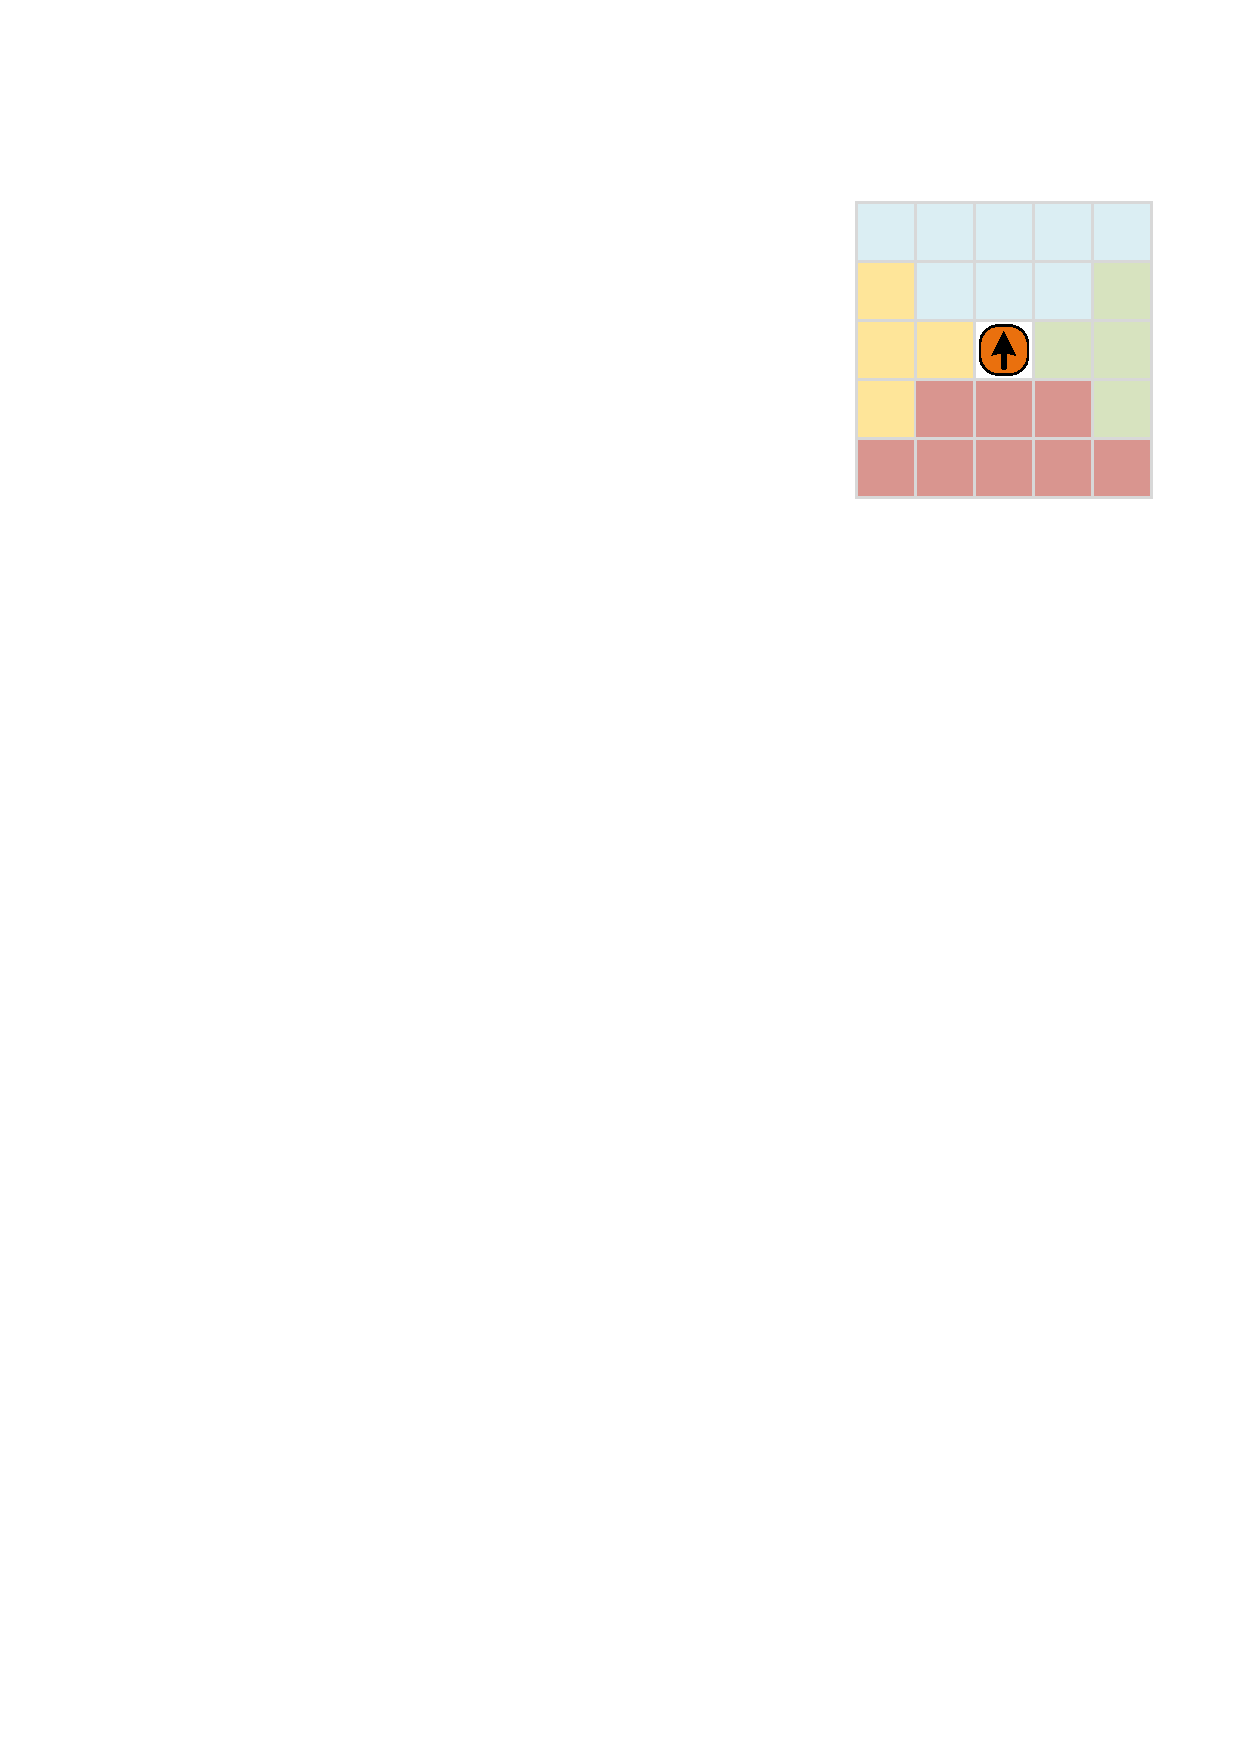
\includegraphics[scale=0.75]{targetdirection_station}
		\caption{Richtungsangaben für Roboter, die sich innerhalb einer Station befinden.}
		\label{fig:targetdirection_1}
	\end{subfigure}
	~~~~~
	\begin{subfigure}[b]{0.6\textwidth}
		\centering
		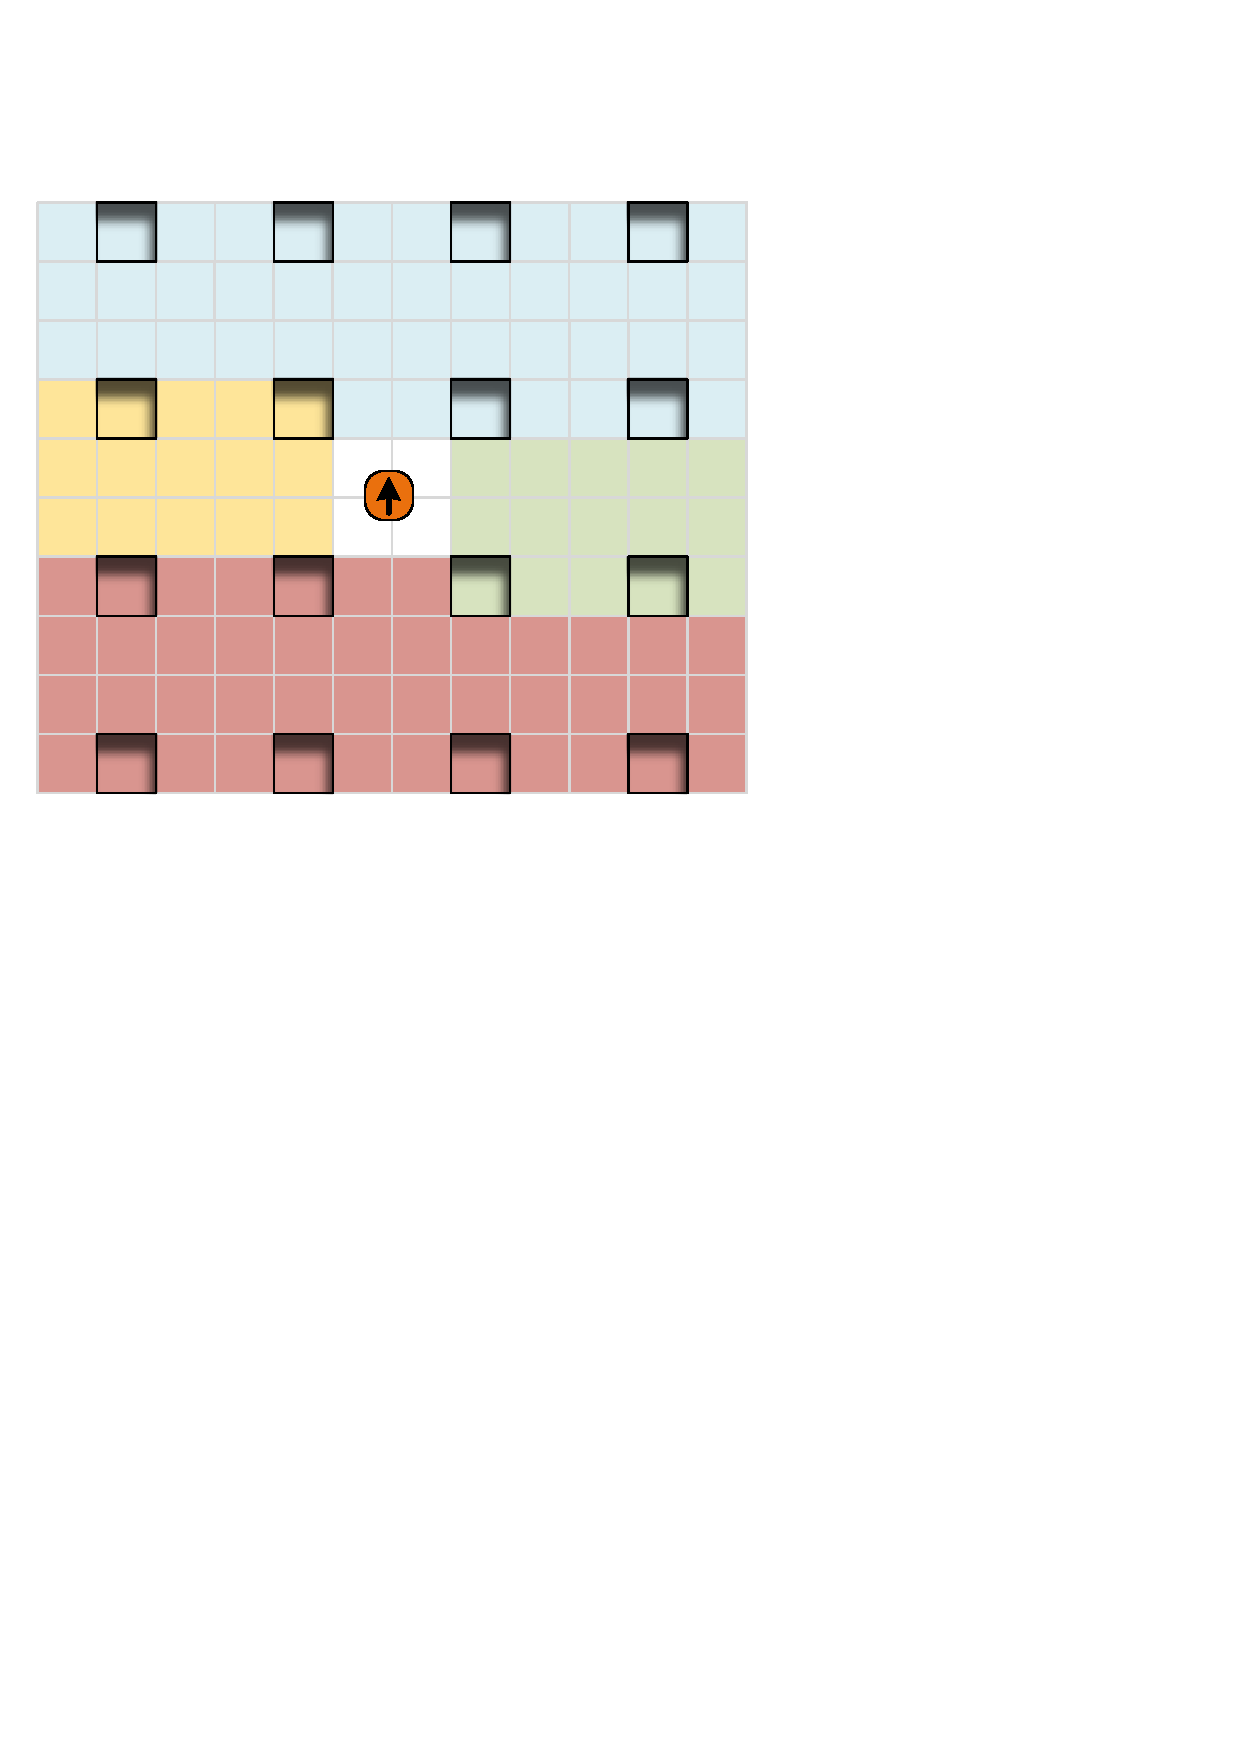
\includegraphics[scale=0.75]{targetdirection_crossroad}
		\caption{Richtungsangaben für Roboter, die sich auf einer Kreuzung befinden.}
		\label{fig:targetdirection_2}
	\end{subfigure}
	\begin{subfigure}[b]{1\textwidth}
		\centering
		\vspace{1cm}
		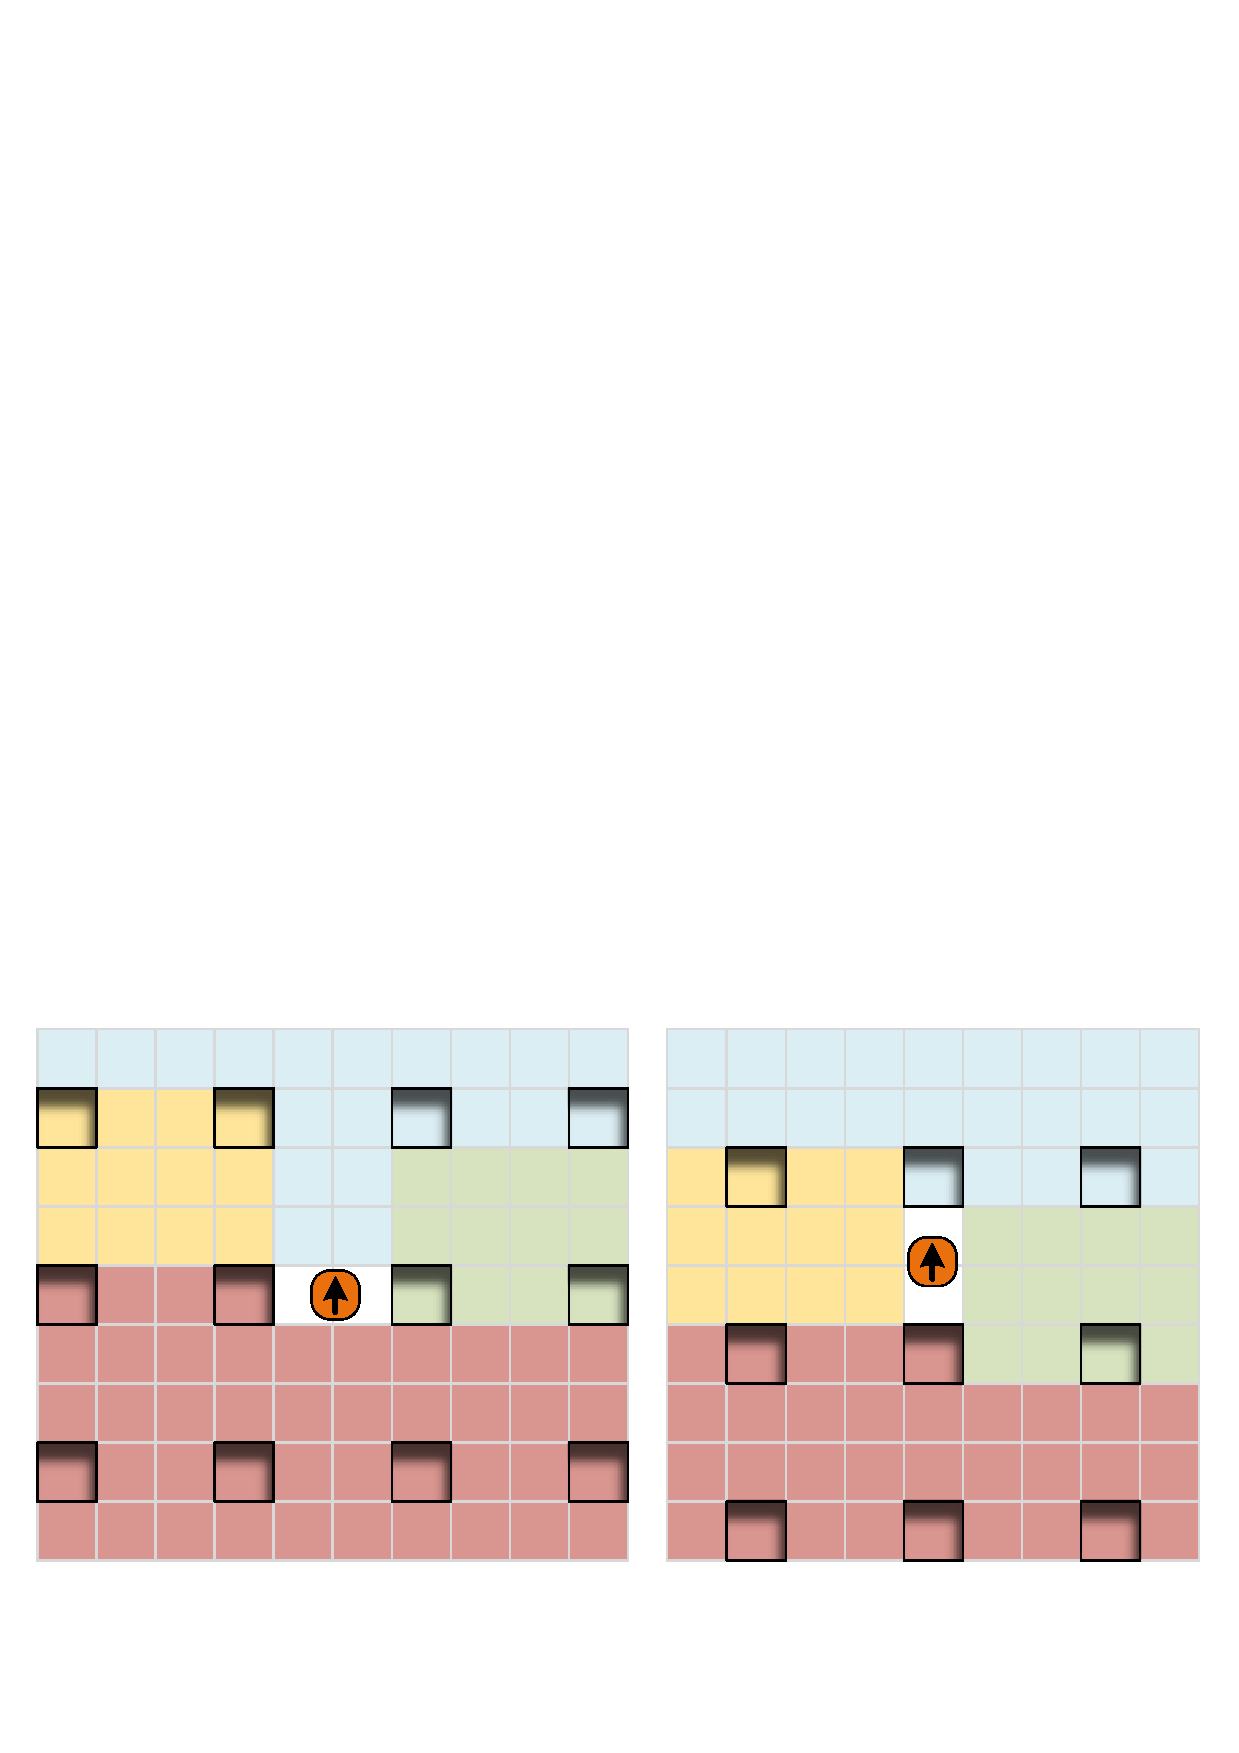
\includegraphics[scale=0.75]{targetdirection_waypoint}
		\caption{Richtungsangaben für Roboter, die sich auf einem Wegpunkt befinden.}
		%Ist der Roboter zu einer Kreuzung hin ausgerichtet, wird diese als \texttt{AHEAD} angesehen, während alle anderen Felder so betrachtet werden als würde der Roboter auf dieser Kreuzung stehen.
		\label{fig:targetdirection_3}
	\end{subfigure}
	\caption{Schematische Darstellung der Rückgaben von der \nameref{method:targetdirection} abhängig vom Standort des Roboters und des Ziels. 
	In den Grafiken symbolisiert blau \texttt{AHEAD}, rot \texttt{BEHIND}, gelb \texttt{LEFT} und grün \texttt{RIGHT}.}
	\label{fig:targetdirection}
\end{figure}

\clearpage

\subsection*{Einfache Methoden zur Hinderniserkennung }

Mithilfe der einfachen Methoden zur Hinderniserkennung der Klasse \texttt{DataSnapshot} ist es möglich abzufragen, ob eins der direkten Nachbarfelder des Roboters blockiert ist. 
Das Verhalten dieser Methoden ist in \autoref{fig:sensor_1} skizziert.

\subsubsection{Methode \texttt{blockedFront()}}

Die Methode \texttt{blockedFront()} gibt einen \texttt{boolean} zurück. 
Die Rückgabe der Methode ist genau dann wahr, wenn das in Fahrtrichtung voraus liegende Feld (ganz oder teilweise) blockiert ist (durch ein Hindernis, eine Trennwand, einen Abwurfschacht oder einen anderen Roboter). 
Siehe auch \autoref{fig:sensor_1}.


\subsubsection{Methode \texttt{blockedLeft()}}

Die Methode \texttt{blockedLeft()} gibt einen \texttt{boolean} zurück. 
Die Rückgabe der Methode ist genau dann wahr, wenn das in Fahrtrichtung links liegende Feld (ganz oder teilweise) blockiert ist (durch ein Hindernis, eine Trennwand, einen Abwurfschacht oder einen anderen Roboter). 
Siehe auch \autoref{fig:sensor_1}.


\subsubsection{Methode \texttt{blockedRight()}}

Die Methode \texttt{blockedRight()} gibt einen \texttt{boolean} zurück. 
Die Rückgabe der Methode ist genau dann wahr, wenn das in Fahrtrichtung rechts liegende Feld (ganz oder teilweise) blockiert ist (durch ein Hindernis, eine Trennwand, einen Abwurfschacht oder einen anderen Roboter). 
Siehe auch \autoref{fig:sensor_1}.



% Zusätzlich gibt es weitere Zugriffsmethoden, die speziell auf den Verkehr in der Sortieranlage ausgelegt sind und gezielt überprüfen, ob Kreuzungen und Wegpunkten von einem anderen Roboter blockiert werden. In \autoref{fig:sensor} ist die designierte Nutzung von \texttt{blockedWaypoint*()} und \texttt{blockedCrossroad*()} visualisiert.

% Mit \texttt{blockedCrossroadAhead()} wird die voraus liegende Kreuzung überprüft (siehe \autoref{fig:sensor_3}) \emph{oder} der \enquote{Rest} der aktuell selbst befahrenen Kreuzung (siehe \autoref{fig:sensor_2}). Mit \texttt{blockedCrossroadRight()} (siehe \autoref{fig:sensor_4}) die Kreuzung zu rechten des Roboters überprüft. Letztere Überprüfung ist relevant, wenn der Roboter die Spur wechseln will.

% Wegpunkte werden mittels den drei \texttt{blockedWaypoint*()}-Methoden überprüft.
% Wenn der Roboter sich dabei selbst auf einem Wegpunkt mit Blick auf eine Kreuzung befindet befindet, werden die Wegpunkt-Positionen erfasst, die ebenfalls auf die Kreuzung einfahren könnten (siehe \autoref{fig:sensor_3}). Befindet er sich auf einer Kreuzung, werden die abgehenden Wegpunkte erfasst, die der Roboter nach verlassen der Kreuzung erreichen würde (siehe \autoref{fig:sensor_2}).

% Sämtliche \texttt{blockedWaypoint*()} und \texttt{blockedCrossroad*()}-Methoden agieren dabei nach dem Prinzip \enquote{garbage in, garbage out}, wenn sie außerhalb der designierten Positionen genutzt werden. 

\subsection*{Komplexe Methoden zur Hinderniserkennung}

Mithilfe der komplexen Methoden zur Hinderniserkennung der Klasse \texttt{DataSnapshot} ist es möglich das Fahrverhalten auf Kreuzungen und Wegpunkten zu definieren. 
%Die komplexen Methoden zur Hinderniserkennung der Klasse \texttt{DataSnapshot} unterstützen das Fahrverhalten zwischen Kreuzungen und Wegpunkten.
Dabei wird die deutsche Straßenverkehrsordnung, konkret der Rechtsverkehr, besonders berücksichtigt.

Die Methoden sind kontextsensitiv, d.h. je nach Position des Roboters werden verschiedene Rückgaben geliefert.
Ist der Roboter auf einem Feld, bei dem eine bestimmte Abfragemethode unpassend ist, funktioniert diese Methode nach dem Prinzip \enquote{Garbage in, Garbage out}. 
So ist es z.B. nicht sinnvoll definiert, welche Rückgabe die Methode \texttt{blockedCrossroadAhead()} innerhalb einer Station liefert.


\begin{figure}[h]
	\centering
	\begin{subfigure}[b]{0.45\textwidth}
		\centering
		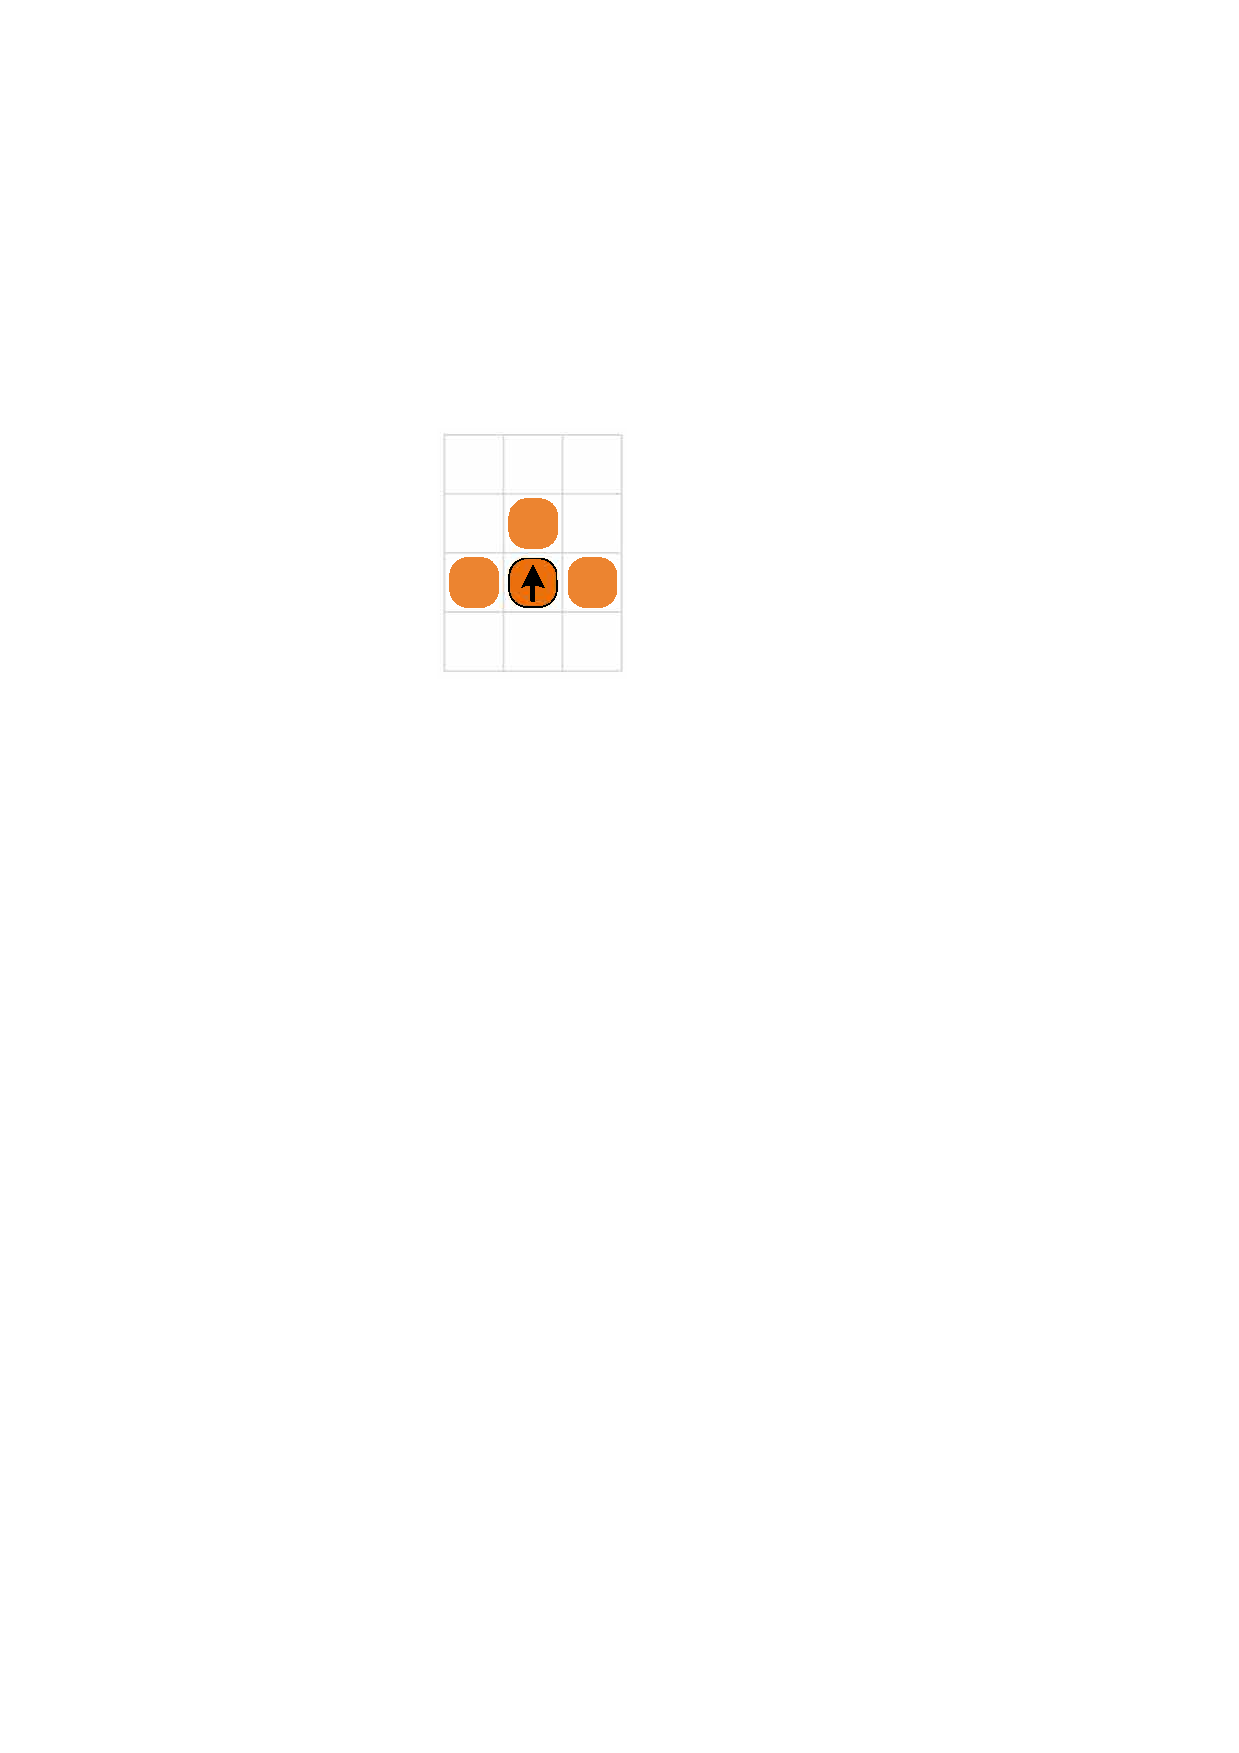
\includegraphics[scale=0.9]{sensor_1}
		\caption{Hindernisabfrage der direkt benachbarten Felder mit den Methoden \texttt{blocked*()}. Grund für eine Blockade können Hindernisse, Trennwände, Abwurfschächte und andere Roboter sein.}
		\label{fig:sensor_1}
	\end{subfigure}
	~~~~~
	\begin{subfigure}[b]{0.45\textwidth}
		\centering
		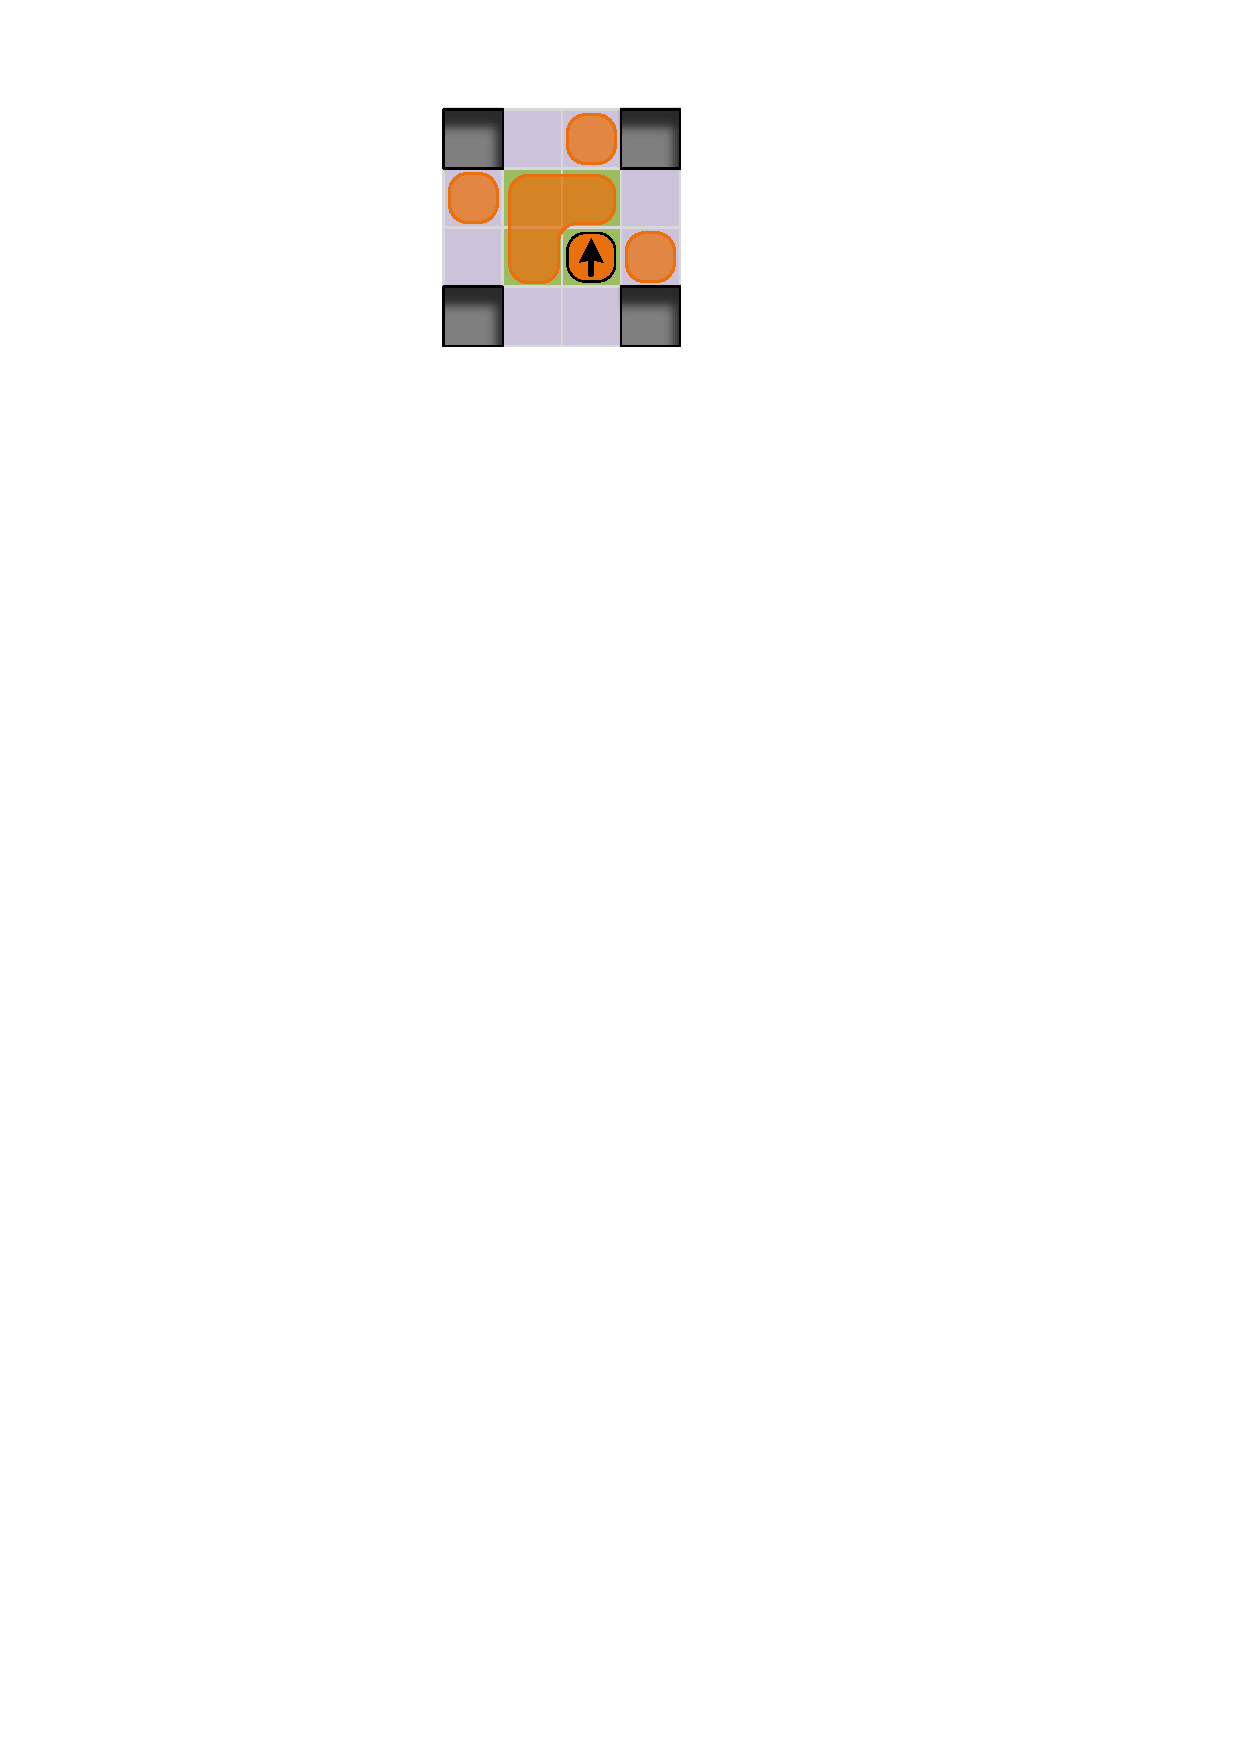
\includegraphics[scale=0.9]{sensor_2}
		\caption{Für Roboter auf einer Kreuzung: Hindernisabfrage der benachbarten Wegpunkte mit den Methoden \texttt{blockedWaypoint*()} und \texttt{blockedCrossroadAhead()} ausgehend von dem unten rechts liegenden Feld einer Kreuzung.}
		\label{fig:sensor_2}
	\end{subfigure}
	\begin{subfigure}[b]{0.45\textwidth}
		\centering
		\vspace{1cm}
		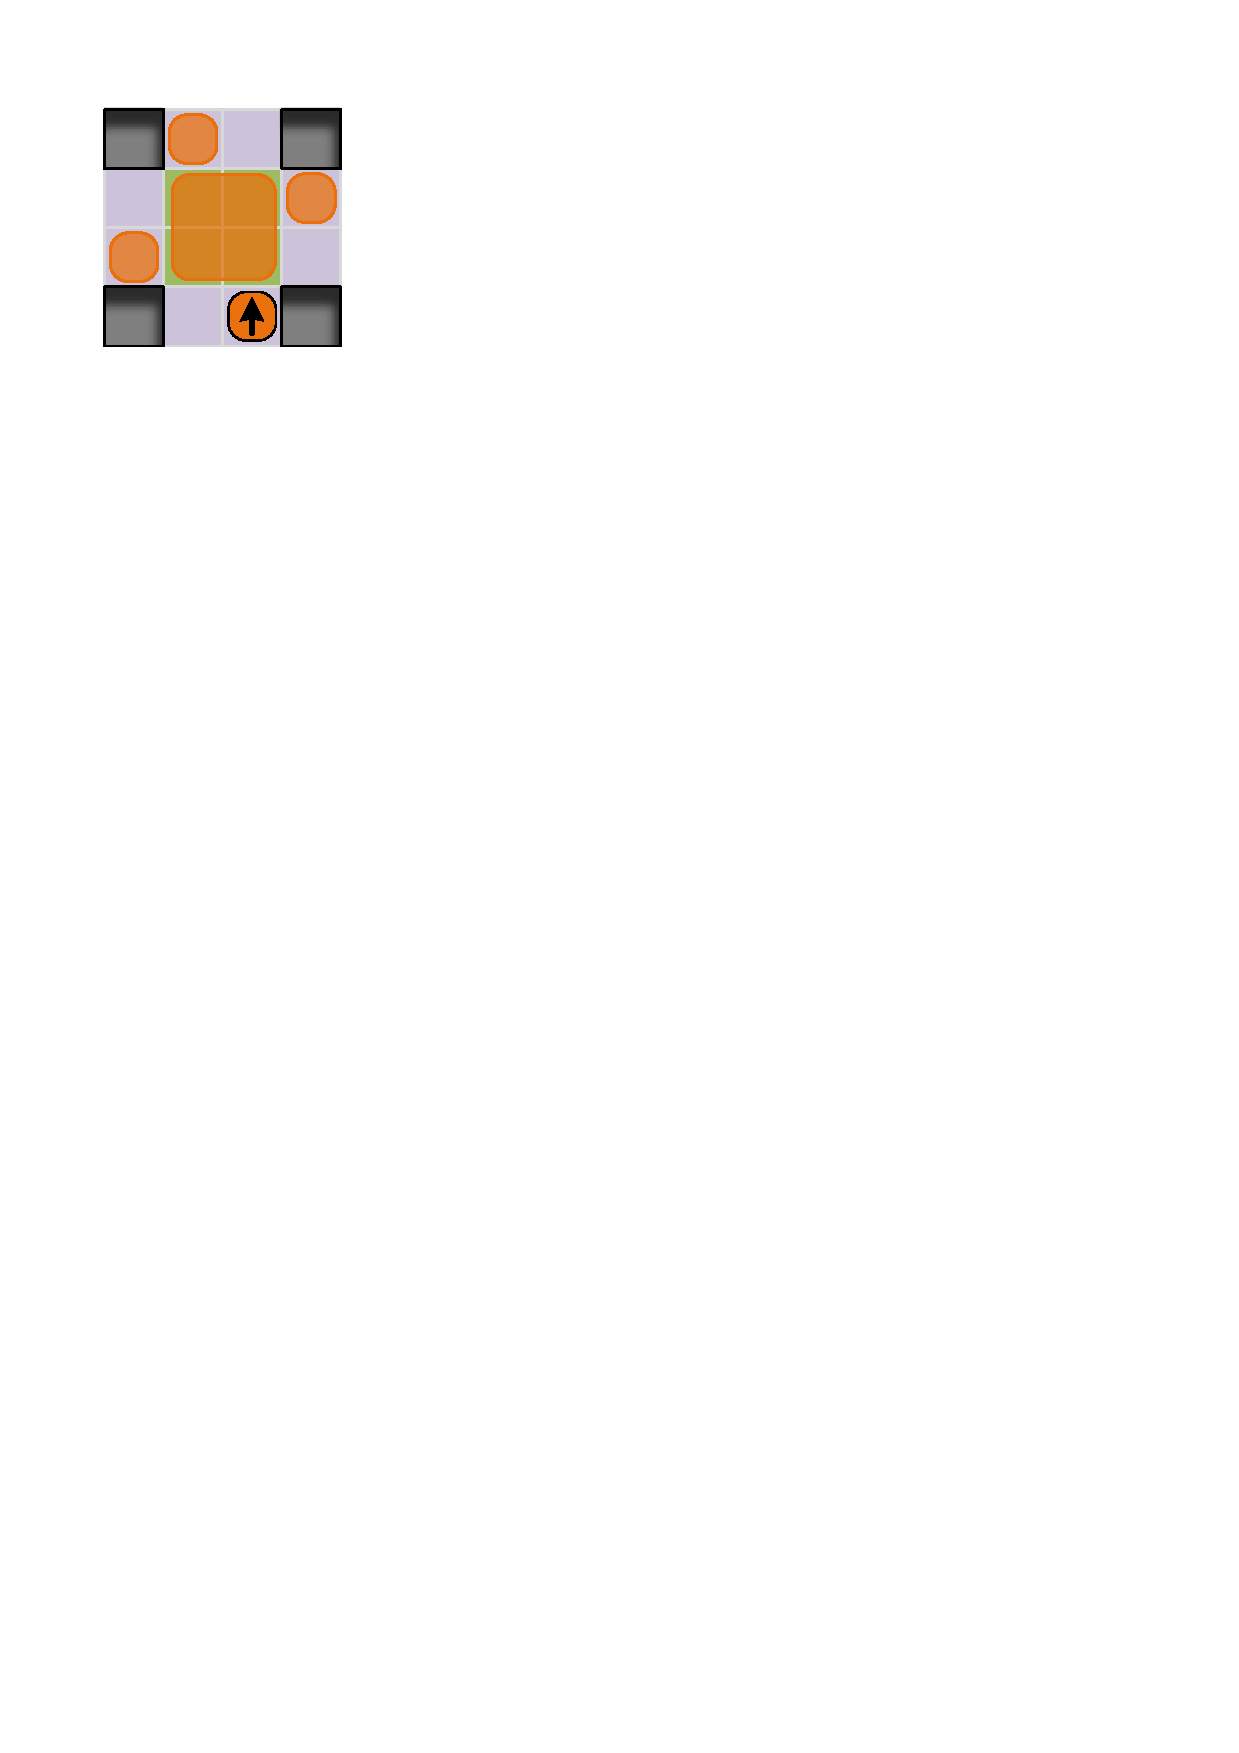
\includegraphics[scale=0.9]{sensor_3}
		\caption{Für Roboter auf einem Wegpunkt: Hindernisabfrage für eine voraus liegende Kreuzung mit der Methode \texttt{blockedCrossroadAhead()} sowie für die dahinter liegenden Wegpunkte mit den Methoden \texttt{blockedWaypoint*()}.}
		\label{fig:sensor_3}
	\end{subfigure}
	~~~~~
	\begin{subfigure}[b]{0.45\textwidth}
		\centering
		\vspace{1cm}
		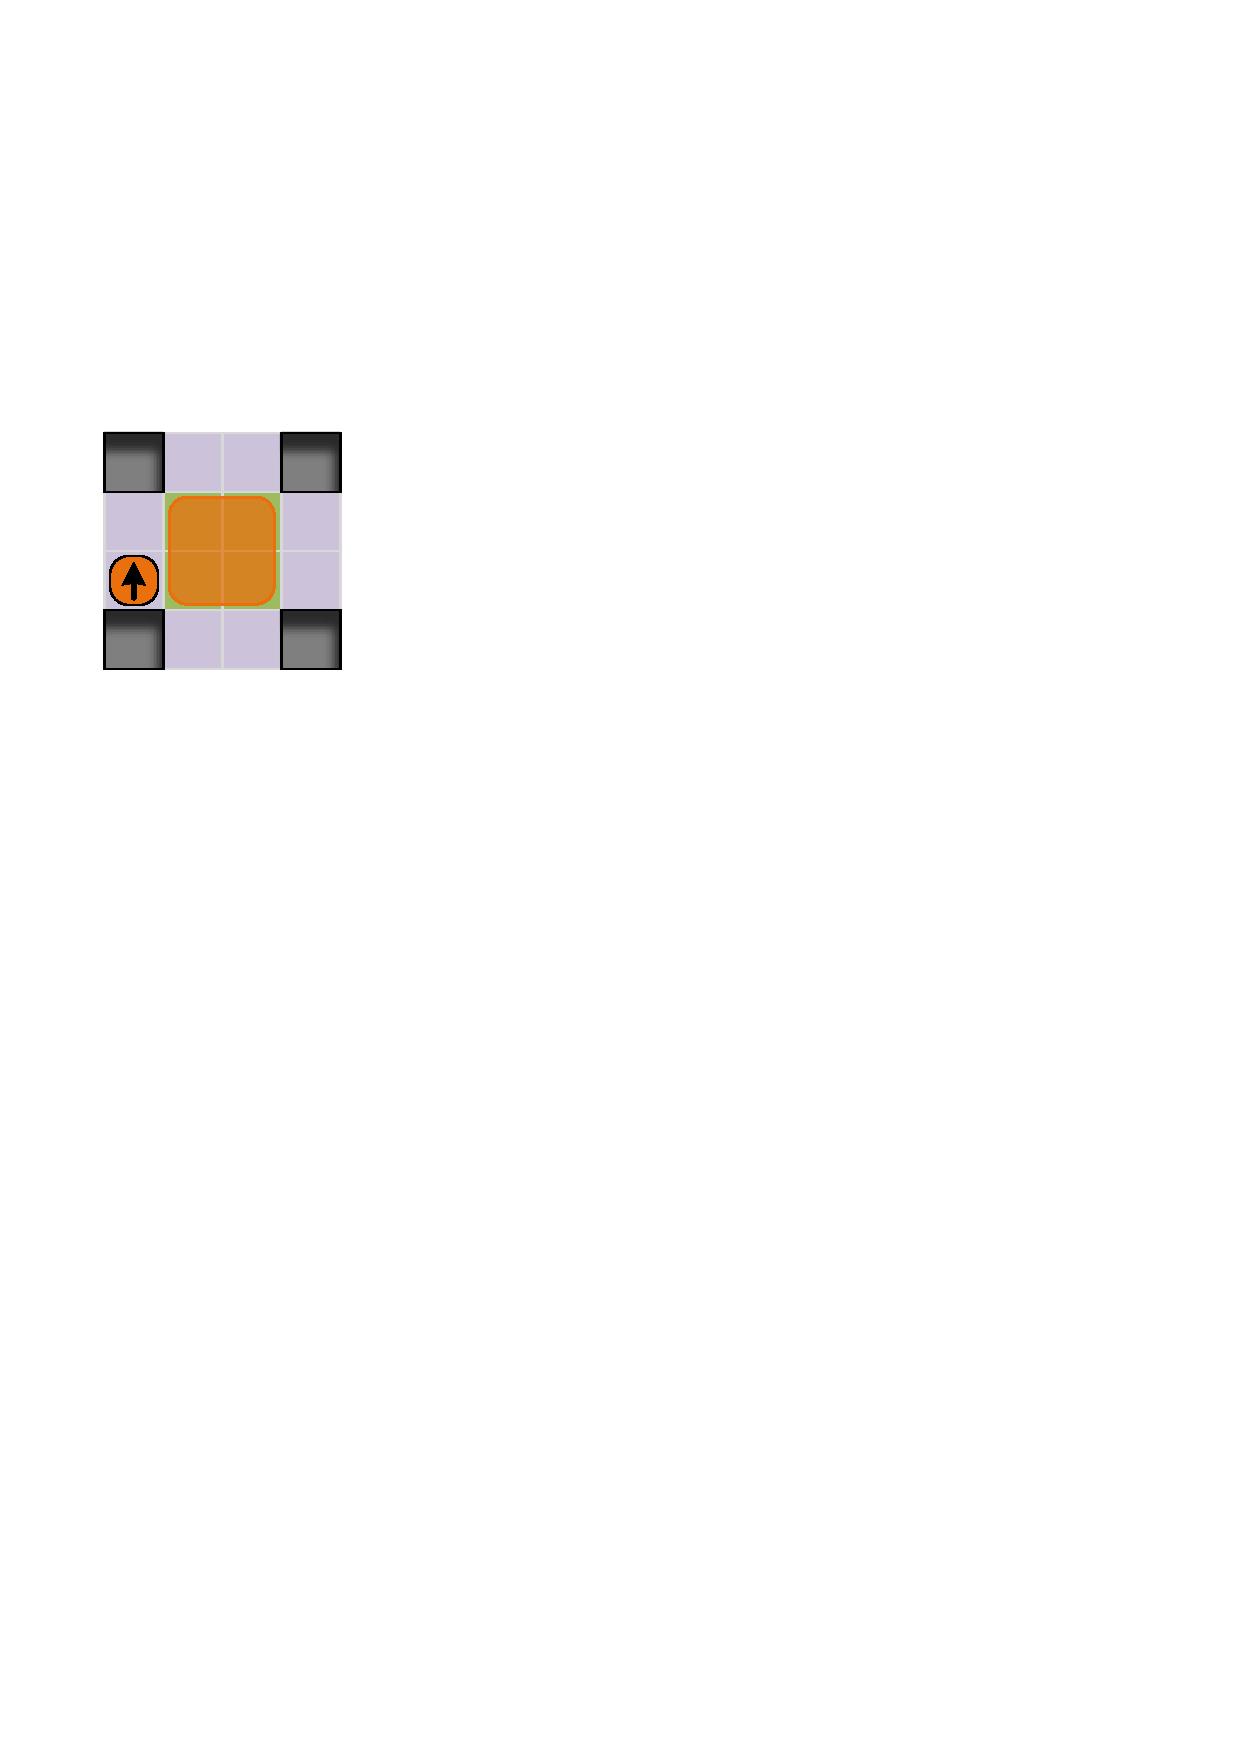
\includegraphics[scale=0.9]{sensor_4}
		\caption{Für Roboter auf einem Wegpunkt: Hindernisabfrage für eine rechts liegende Kreuzung mit der Methode \texttt{blockedCrossroadRight()}.} % Ist diese Kreuzung leer kann garantiert werden, dass kein anderer Roboter das voraus liegende Feld erreichen kann.}
		\label{fig:sensor_4}
		\vfill{}
	\end{subfigure}
	\caption{Funktionsweise der (einfachen und komplexen) Methoden zur Hinderniserkennung, die es der Klasse \texttt{DataSnapshot} ermöglichen zu prüfen, ob Felder in der Umgebung des Roboters blockiert sind.}
	\label{fig:sensor}
\end{figure}

\clearpage

\subsubsection{Methode \texttt{blockedWaypointAhead()}}

Die Methode \texttt{blockedWaypointAhead()} gibt einen \texttt{boolean} zurück.

Befindet sich der Roboter auf einem Wegpunkt mit Blick auf eine Kreuzung, gibt die Methode \texttt{blockedWaypointAhead()} genau dann wahr zurück, wenn ein anderer Roboter auf dem gegenüberliegenden Wegpunkt so steht, dass er (gemäß Rechtsverkehr) in die Kreuzung einfahren könnte (siehe \autoref{fig:sensor_2}).

Befindet sich der Roboter auf einer Kreuzung, wird dagegen geprüft, ob ein anderer Roboter so auf dem gegenüberliegenden Wegpunkt steht, dass der Roboter selbst die Kreuzung nicht verlassen kann (siehe \autoref{fig:sensor_3}).


\subsubsection{Methode \texttt{blockedWaypointLeft()}}

Die Methode \texttt{blockedWaypointLeft()} gibt einen \texttt{boolean} zurück.

Befindet sich der Roboter auf einem Wegpunkt mit Blick auf eine Kreuzung, gibt die Methode \texttt{blockedWaypointLeft()} genau dann wahr zurück, wenn ein anderer Roboter auf dem in Fahrtrichtung links liegenden Wegpunkt so steht, dass er (gemäß Rechtsverkehr) in die Kreuzung einfahren könnte (siehe \autoref{fig:sensor_2}).

Befindet sich der Roboter auf einer Kreuzung, wird dagegen geprüft, ob ein anderer Roboter so auf dem links liegenden Wegpunkt steht, dass der Roboter selbst die Kreuzung nicht verlassen kann (siehe \autoref{fig:sensor_3}).


\subsubsection{Methode \texttt{blockedWaypointRight()}}

Die Methode \texttt{blockedWaypointRight()} gibt einen \texttt{boolean} zurück.

Befindet sich der Roboter auf einem Wegpunkt mit Blick auf eine Kreuzung, gibt die Methode \texttt{blockedWaypointRight()} genau dann wahr zurück, wenn ein anderer Roboter auf dem in Fahrtrichtung rechts liegenden Wegpunkt so steht, dass er (gemäß Rechtsverkehr) in die Kreuzung einfahren könnte (siehe \autoref{fig:sensor_2}).

Befindet sich der Roboter auf einer Kreuzung, wird dagegen geprüft, ob ein anderer Roboter so auf dem rechts liegenden Wegpunkt steht, dass der Roboter selbst die Kreuzung nicht verlassen kann (siehe \autoref{fig:sensor_3}).

\enlargethispage{1\baselineskip}

\subsubsection{Methode \texttt{blockedCrossroadAhead()}}

Die Methode \texttt{blockedCrossroadAhead()} gibt einen \texttt{boolean} zurück.

Befindet sich der Roboter auf einem Wegpunkt mit Blick auf eine Kreuzung, gibt die Methode \texttt{blockedCrossroadAhead()} genau dann wahr zurück, wenn die Kreuzung durch mindestens einen anderen Roboter blockiert ist (siehe \autoref{fig:sensor_2}).

Ist der Roboter bereits auf einer Kreuzung, gibt die Methode \texttt{blockedCrossroadAhead()} wahr zurück, wenn auf mindestens einem anderen Feld dieser Kreuzung bereits ein Roboter steht. 
Dabei darf der Roboter sich selbst nicht als Blockadegrund wahrnehmen (siehe \autoref{fig:sensor_3}).


\subsubsection{Methode \texttt{blockedCrossroadRight()}}

Die Methode \texttt{blockedCrossroadRight()} gibt einen \texttt{boolean} zurück.
Die Rückgabe der Methode ist genau dann wahr, wenn die rechts vom Roboter liegende Kreuzung durch mindestens einen anderen Roboter blockiert ist (siehe \autoref{fig:sensor_4}).





\end{document}



